\documentclass[12pt,]{article}
\usepackage{lmodern}
\usepackage{amssymb,amsmath}
\usepackage{ifxetex,ifluatex}
\usepackage{fixltx2e} % provides \textsubscript
\ifnum 0\ifxetex 1\fi\ifluatex 1\fi=0 % if pdftex
  \usepackage[T1]{fontenc}
  \usepackage[utf8]{inputenc}
\else % if luatex or xelatex
  \ifxetex
    \usepackage{mathspec}
  \else
    \usepackage{fontspec}
  \fi
  \defaultfontfeatures{Ligatures=TeX,Scale=MatchLowercase}
\fi
% use upquote if available, for straight quotes in verbatim environments
\IfFileExists{upquote.sty}{\usepackage{upquote}}{}
% use microtype if available
\IfFileExists{microtype.sty}{%
\usepackage{microtype}
\UseMicrotypeSet[protrusion]{basicmath} % disable protrusion for tt fonts
}{}
\usepackage[margin=1in]{geometry}
\usepackage{hyperref}
\hypersetup{unicode=true,
            pdftitle={Sending a Balloon to the Edge of Space},
            pdfauthor={Luker Bowsher, John Kim, Vivian Liu, Simon Oros, Caroline Pang, Alec Vercruysse},
            pdfborder={0 0 0},
            breaklinks=true}
\urlstyle{same}  % don't use monospace font for urls
\usepackage{longtable,booktabs}
\usepackage{graphicx,grffile}
\makeatletter
\def\maxwidth{\ifdim\Gin@nat@width>\linewidth\linewidth\else\Gin@nat@width\fi}
\def\maxheight{\ifdim\Gin@nat@height>\textheight\textheight\else\Gin@nat@height\fi}
\makeatother
% Scale images if necessary, so that they will not overflow the page
% margins by default, and it is still possible to overwrite the defaults
% using explicit options in \includegraphics[width, height, ...]{}
\setkeys{Gin}{width=\maxwidth,height=\maxheight,keepaspectratio}
\usepackage[normalem]{ulem}
% avoid problems with \sout in headers with hyperref:
\pdfstringdefDisableCommands{\renewcommand{\sout}{}}
\setlength{\emergencystretch}{3em}  % prevent overfull lines
\providecommand{\tightlist}{%
  \setlength{\itemsep}{0pt}\setlength{\parskip}{0pt}}
\setcounter{secnumdepth}{5}
% Redefines (sub)paragraphs to behave more like sections
\ifx\paragraph\undefined\else
\let\oldparagraph\paragraph
\renewcommand{\paragraph}[1]{\oldparagraph{#1}\mbox{}}
\fi
\ifx\subparagraph\undefined\else
\let\oldsubparagraph\subparagraph
\renewcommand{\subparagraph}[1]{\oldsubparagraph{#1}\mbox{}}
\fi

%%% Use protect on footnotes to avoid problems with footnotes in titles
\let\rmarkdownfootnote\footnote%
\def\footnote{\protect\rmarkdownfootnote}

%%% Change title format to be more compact
\usepackage{titling}

% Create subtitle command for use in maketitle
\newcommand{\subtitle}[1]{
  \posttitle{
    \begin{center}\large#1\end{center}
    }
}

\setlength{\droptitle}{-2em}

  \title{Sending a Balloon to the Edge of Space}
    \pretitle{\vspace{\droptitle}\centering\huge}
  \posttitle{\par}
    \author{Luker Bowsher, John Kim, Vivian Liu, Simon Oros, Caroline Pang, Alec
Vercruysse}
    \preauthor{\centering\large\emph}
  \postauthor{\par}
      \predate{\centering\large\emph}
  \postdate{\par}
    \date{November 13, 2018}

\usepackage{setspace}
\usepackage{gensymb}
\usepackage{pdfpages}

\begin{document}
\maketitle
\begin{abstract}
This paper details 6thsense, a mission to send a weather balloon to to
edge of space in order to study Earth's atmosphere. The weather balloon
is outfitted with a payload that includes a camera, inside and outside
temperature sensors, a barometer, multiple GPS tracking devices, as well
as a host of individual experiments. The balloon most likely reached an
altitude of 20,000 meters, into the stratosphere and ozone layer. The
balloon was successfully recovered after approximately one and one half
hours of flight.
\end{abstract}

\newpage

\setcounter{secnumdepth}{3} \setcounter{tocdepth}{3} \tableofcontents
\newpage
\onehalfspacing

\section{Introduction}\label{introduction}

\subsection{Background}\label{background}

There are four main layers to the atmosphere: the troposphere,
stratosphere, mesosphere, and thermosphere. The \textbf{troposphere} is
the section of the atmosphere from roughly 0km to 15km, and is the layer
in which humans live. It includes 75\% of the mass of all gases in the
atmosphere, consisting of 78\% nitrogen gas, 21\% oxygen, and less than
1\% of argon, carbon dioxide, and other constituents. Because it is both
the lowest in altitude and most massive layer, the pressure in the
troposphere is the greatest: 100kPa. As altitude increases in the
troposphere, temperature decreases to about -60 \degree C. The**
stratosphere** is the section from roughly 15km to 50km. The ozone
layer, or the region in the atmosphere which absorbs most UV rays, is
within the stratosphere at about 20km in altitude. The pressure in the
stratosphere is 10kPa. The mesosphere is the region from 50km to 80km.
The pressure in the mesosphere is 0.1 kPa. Finally, the thermosphere is
the highest in altitude of the four layers, spanning from 80km into
outer space. Here, the pressure is only 0.01kPa, as it is the least
dense of the layers. The few air molecules in the thermosphere are
heated to extremely high temperatures by the Sun's radiation. However,
because there are so few molecules, an appreciable difference in overall
temperature cannot be measured, so the effective temperature of the
thermosphere is less than that of the mesosphere.

The layers relevant to the experiments conducted are the troposphere and
stratosphere, as the balloon was designed to reach a maximum altitude of
30km (about the middle of the stratosphere but past the ozone layer).
Therefore, the payload had to prepared for temperatures as low as -60
\degree C and pressure as low as 10kPa (in the stratosphere). The
payload is expected to encounter the lowest temperature in the
troposphere, around an altitude of 10km. As the balloon rises from sea
level to the top of the troposphere, temperature is expected to decrease
because the ground absorbs most of the sun's radiation (as opposed to
the gas particles). However, as the balloon enters the stratosphere, an
increase in temperature is expected due to the ozone layer's blockage of
UV rays. The UV rays that the ozone layer absorbs causes the gas
particles in the stratosphere to heat up, so temperature increases with
altitude. As the balloon gains altitude, the density of air around it
decreases, so the pressure decreases.

\subsection{Greenhouse Gases in the
Atmosphere}\label{greenhouse-gases-in-the-atmosphere}

The presence of greenhouse gasses in the atmosphere contribute to the
warming of the earth's surface and the troposphere because of the
greenhouse effect. The greenhouse effect describes the trapping of heat
within the earth's atmosphere via the infrared absorption of certain
molecules.

When infrared radiation enters the atmosphere, short-wave infrared
radiation (700 - 1000 nm) does not effectively interact with greenhouse
gasses. The photons instead pass through the atmosphere and reach the
surface of the earth. Here, they are absorbed by the surface of the
earth and get reemitted as a lower energy, longer-waved infrared photon.
Greenhouse gasses can now absorb these lower energy photons and reemit
them. This absorption and reemission warms the troposphere by increasing
the kinetic energy the atmosphere. Additionally, greenhouse gasses can
reemit photons back towards the surface of the earth, increasing the
temperature of the earth's surface. By impeding the tendency for
long-wave radiation to leave the atmosphere, the greenhouse effect
increase the temperature of the troposphere and surface. (Britannica,
2018)

The spectroscopy that explains the greenhouse effect concerns molecular
vibration. Infrared photons excite vibrations in molecules. Since the
vibrational frequency of atoms are quantized, only certain energies will
excite vibration in a molecule. Different molecules can exhibit
different vibrational modes. A molecule with more atoms has more
vibrational modes. The infrared selection rule states that a vibrational
mode is active when it is changing the dipole moment of the molecule. An
active vibrational mode is a molecular vibration that can be excited by
an infrared photon. Thus, infrared photons will only be absorbed when
that molecule's dipole moment is changing. (Pecsok, 1968) Molecules such
as nitrogen and oxygen will never exhibit a change in their dipole
moment due to vibration because their only vibrational mode involves the
singular oscillation of the distance between two atoms. Thus, they
cannot absorb infrared radiation in order to partake in the greenhouse
effect and are not considered greenhouse gasses. On the other hand, many
atmospheric molecules that have more than two atoms have more complex
vibrational modes. These active vibrational mode gasses, such as
nitrogen dioxide and water, are called greenhouse gasses. (UCAR, 2012)

As the greenhouse effect warms the planet, many factors accelerate the
temperature rise by creating positive feedback loops. Positive feedback
loops amplify any global increase in temperature. One positive feedback
loop is created when rising temperatures melt glaciers. These white and
reflective icy surfaces melt into dark oceans which absorb more
radiation and heat up faster. This explains the approaching transition
from a permanent to a seasonal ice cover in the Arctic Ocean. Thus
temperature increases accelerate. (Kashiwase, 2017)

Another positive feedback loop involves the melting of permafrost. A
quarter of the northern hemisphere is covered in permafrost that holds
concentrated methane and carbon dioxide. Slight growths in temperature
are enough to thaw the permafrost. When it melts, these greenhouse
gasses are released into the atmosphere. Thus, the greenhouse effect
amplifies and global temperature growth accelerates. (Vaks, 2013)

Finally, humidity is also a positive feedback loop. As global
temperatures rise, the atmosphere can hold more water vapor because less
of it gets condensed. Water vapor is a greenhouse gas itself. Thus any
increase in global temperatures will be amplified due to the water vapor
positive feedback loop.

The annual increase of atmospheric carbon dioxide concentration is
approximately 100 times greater in the past 60 years than it has been
during any previous natural increase (Lindsey, 2018). Additionally,
methane concentrations have more than doubled since the start of the
industrial revolution (Britannica, 2018). Partly due to the increase of
these gas concentration along with many positive feedback loops, the
planet's average surface temperature has risen 0.9\degree C since the
late 19th century (Lindsey). With rising temperatures comes the
consequences of severe weather patterns, flooding and other natural
disasters. Collecting atmospheric data of things such as temperature and
gas concentrations informs our understanding of the progression of the
greenhouse effect. With this information, methods can be researched and
developed to impede rising global temperatures.

The Panel on Climate Change has recognized that as global temperatures
rise, lightning strikes will occur more frequently. As skyscrapers get
higher and multiply, lightning strike sourced Terrestrial Gamma ray
Flashes (TGF) become a concern.

TGFs are short, powerful bursts of gamma rays detected in the
atmosphere. Each burst contains 10\^{}17 to 10\^{}19 gamma rays and last
about 1 ms. They were first detected in the 1950s. The United States,
concerned with the Soviet Union's nuclear progress used satellites to
detect gamma rays and track the enemy's progress. After observing long,
5-10 second gamma ray glows (suspected to be Gamma ray Bursts (GRB) from
stars), the U.S. sent more satellites to explore GRB further. In
addition to detecting GRB, the data from these satellites led to the
discovery of TGFs. When short, gamma ray bursts were analyzed for their
source locations, researchers noticed that these burst mainly came from
coastal sites on the equator. After recognizing a correlation with
lightning prone areas and these short gamma ray bursts, C. T. R.
Wilson's theory concerning a Relativistic Runaway Electron Avalanche
(RREA) was applied to discover TGFs.

Wilson's RREA theory relies on a quantum properties of electrons. As the
velocity of normal objects traveling through the atmosphere increases,
the air resistance increases also. Therefore, in a constant force field,
the object will reach a terminal velocity. For electrons however, while
the air resistance initially increase with its speed, at high
velocities, the air resistance on the electron begins to decrease. This
is because at relativistic speeds, the electron can avoid interactions
with other molecules. Thus, after the electron reaches a certain speed,
it will never reach a terminal velocity and accelerate indefinitely as
long as it is still in a force field. Electrons that escape terminal
velocity are called runaway electrons. The second part of Wilson theory
involves an explanation of the ``Avalanche.'' Runaway electrons can
knock other electrons while accelerating and cause them to become
runaway electrons also. This creates an exponential increase of runaway
electrons as more and more electrons interact.

The RREA theory explains a hypothesis for TGFs. The field that
accelerates runaway electrons is an electric field produced by the
separation of charges in thunderclouds. The energy field required to
cause a RREA is powerful enough to cause lightning strikes. Thus, the
occurrence of a lightning strike is correlated with that of a TGF. As
electrons accelerate through the atmosphere, they can undergo
Bremsstrahlung interactions with the nucleuses of air molecules. When an
electron is deflected around a nucleus, a powerful Bremsstrahlung photon
is emitted. Since an avalanche of electrons undergo this interaction,
this explains the massive quantity of gamma rays contained in one TGF.

While there is an abundance of research done on upward directed TGFs
(those detected by the satellites in the 1950s), there is a lack of data
detecting downward directed TGFs. Currently, researchers led by David M.
Smith at UC Santa Cruz and other researchers around the world are using
a multitude of methods to detect downwards directed TGFs. Some methods
include sending detectors in cargo planes, on weather balloons and on
the ground in thunder prone areas. Since TGFs are so powerful, detectors
usually fail if they are near a TGF because of the sheer amount of
energy exerted. This field of research is relatively new and active.
(Smith, 2015)

\subsection{Empirical and Exponential Models for Temperature and
Pressure}\label{empirical-and-exponential-models-for-temperature-and-pressure}

\begin{figure}[h]

{\centering 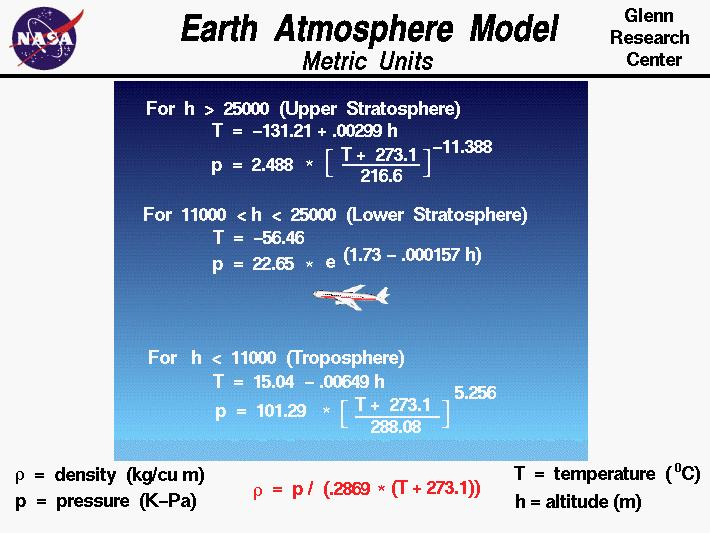
\includegraphics{assets/nasa_model} 

}

\caption{\label{fig:figs} NASA Empirical Models for Temperatur and Pressure}\label{fig:NASA_image}
\end{figure}

Figure 1 shows NASA's empirical models for pressure and temperature for
the troposphere and stratosphere. For a height of 0, the temperature is
that of sea level, or 15.06 \degree C. At a height of 11km, the
predicted temperature is -56.35 \degree C, which is consistent with
measurements recorded by the payload. As the balloon rises through the
lower stratosphere, a constant temperature of -56.46 \degree C is
expected. Finally, once the balloon rises beyond the ozone layer (around
25km altitude), temperatures are expected to rise again due to the ozone
layer's absorption of the sun's radiation. Refer to section 8 for an
overlay of NASA's empirical models over experimental data.

\section{Experiments Conducted}\label{experiments-conducted}

The payload included two tracking devices, a GoPro Hero 3+ to record the
ascent, and sensors to monitor the atmosphere and record altitude data.
In addition, each team member implemented a sensor as part of an
individual experiment. This paper focuses on the results of the group
experiments, but the setups for the individual experiments are still
described. Separate papers can be found for each team member's
individual experiment.

\subsection{Group Experiments}\label{group-experiments}

\begin{longtable}[]{@{}lll@{}}
\toprule
Sensor & Function & Model\tabularnewline
\midrule
\endhead
Real Time Clock & Accurate Timing & Sparkfun DS1307 RTC\tabularnewline
GPS & Location Data & Sparkfun Venus GPS\tabularnewline
Barometer & Altitude Data & Vernier Gas Pressure Sensor\tabularnewline
Temperature & Outside Temperature & Adafruit BME280\tabularnewline
Humidity & Outside Humidity & Adafruit BME280\tabularnewline
Temperature & Inside Temperature & Thermistor\tabularnewline
\bottomrule
\end{longtable}

In addition, a PicoAPRS was used to provide live GPS coordinates,
altitude, heading, and speed measurements.

These sensors were picked in order to be able to track the balloon
through its flight and provide baseline measurements to compare other
individual sensors to. By recording accurate altitude and time
measurements with the measurement of every other sensor, sensor data can
be analyzed with respect to both time and altitude. Furthermore,
recording temperature data for both inside and outside the payload helps
provide diagnostic data for if any specific part of the payload fails,
and provides another baseline to compare any other sensor measurements
to. The Humidity sensor not only provides humidity data which can be
analyzed with respect to Altitude, but it can also determine when the
payload is in a cloud, which could affect the measurements of other
sensors.

\subsubsection{How a Pressure Sensor
Works}\label{how-a-pressure-sensor-works}

Most pressure sensors, including the Vernier gas pressure sensor that is
connected to the main Arduino mega board and used on the payload,
measure gas pressure by using a flexible diaphragm, where one side is a
vacuum and the other side is open to the surrounding atmosphere, and
producing a voltage that varies linearly with absolute pressure. A
typical capacitive humidity sensor measures relative humidity by placing
a sheet of metal oxide between two electrodes and measuring the change
in capacitance between the electrodes, which is directly proportional to
the change in air moisture. And lastly, the temperature sensor used in
the following experiments, specifically a thermistor, measures
temperature through nonlinear changes in resistance, which decreases as
temperature increases.

\subsection{Individual Experiments
Conducted}\label{individual-experiments-conducted}

\begin{longtable}[]{@{}ll@{}}
\toprule
Team.Member & Experiment\tabularnewline
\midrule
\endhead
Alec Vercruysse & Spectrometer\tabularnewline
Luke Bowsher & Accelerometer\tabularnewline
Simon Oros & \sout{Geiger Counter}*\tabularnewline
Vivian Liu & Light Intensity Sensors\tabularnewline
Caroline Pang & UVB Sensor\tabularnewline
John Kim & Methane Sensor\tabularnewline
\bottomrule
\end{longtable}

*shortly before launch it was discovered that the Geiger Counter was
non-operable and therefore it was taken out of the payload. Instead,
Simon Oros focused on ground-level radiation measurements.

\subsubsection{Alec Vercruysse:
Spectrometer}\label{alec-vercruysse-spectrometer}

Identifying the gaseous composition of the atmosphere is of great
importance in order to be able to properly analyze the different layers
and their properties. Specifically, identifying the composition of the
ozone layer is extremely important in order to determine its health.
Actively monitoring the ozone layer is crucial, since it is responsible
for shielding life on earth from harmful Ultraviolet light. Furthermore,
analyzing the gaseous composition of the troposphere is important to
understanding and measuring the greenhouse effect (see section 1). The
more greenhouse gasses in the atmosphere, the larger the greenhouse
effect. This leads to more heat trapped in the atmosphere, and
accelerated global warming.

A spectrometer was placed at a 45 \degree angle relative to the top
acrylic plate in order to perform spectral analysis of the atmosphere,
with a view unobstructed by the balloon or payload.

\subsubsection{John Kim: Methane Sensor}\label{john-kim-methane-sensor}

Greenhouse gases are gases that trap heat that come from both the human
activity and the Sun inside the Earth's atmosphere, resulting in global
warming and climate change when overlooked. While many identify
greenhouse gases with carbon dioxide, methane contributes to over 10\%
of the gaseous composition of the atmosphere and is emitted from coal
mining and organic waste. Monitoring methane levels is crucial to not
only furthering the understanding of how the Earth's atmospheric
composition changes over time, but also protecting the
environment---methane is much more efficient than carbon dioxide at
absorbing heat and more potent. Scientists have even written letters to
the United Nations' climate change summit to require nations to curb
methane emissions more quickly.

A methane sensor was placed inside the insulated payload because it was
found to be fairly sensitive to temperature when compared to other
components that were placed outside the styrofoam box. In addition,
there would not have been any significant difference in methane levels
inside and outside the payload because the non-restrictive airflow
inside the box would have allowed methane gas to pass through relatively
unobstructed. A typical methane sensor measures methane gas by detecting
the changes in resistance when the gas comes into contact with a
catalytic surface and heats the wiring resistance.

\subsubsection{Caroline Pang: UVB
Sensor}\label{caroline-pang-uvb-sensor}

Ultraviolet light is a harmful form of radiation which enters our
atmosphere. There are three classifications of ultraviolet radiation,
UVA, UVB, and UVC. The ozone layer is responsible for absorbing most of
the harmful UVC radiation making it an essential part of the atmosphere.
However, it only partially absorbs UVB light which is responsible for
causing sunburns and in extreme cases, skin cancer. Measuring the
intensity of UVB light as a function of altitude and observing how it
changes when entering the ozone layer can demonstrate how effectively
the ozone layer absorbs UVB light.

Therefore, a UVB light sensor was placed vertically inside the payload
with the top half of the rod outside of the acrylic top to measure the
intensity of UVB light.

\subsubsection{Vivian Liu: Light Intensity and Solar
Power}\label{vivian-liu-light-intensity-and-solar-power}

Light intensity, specifically for the purposes of solar energy, is an
important part of the initiative for cleaner energy. It is also
interesting to learn about how light intensity increases or decreases as
it passes through the ozone layer.

To test light intensity, a photoresistor was placed on a board, and the
resistances of the photoresistor attached in series to a 1.2k Ohm
resistor were recorded as a function of altitude. From the resistance of
the photoresistor, lux, or the units of light intensity, can be
calculated. For solar power, the arduino read the voltage of a solar
panel that was placed outside of the shadow of the balloon. From this
voltage, power output of the solar panel can be calculated. The purpose
of the experiments on solar properties is to see if there is a
correlation between altitude and solar output.

\section{Physical Design}\label{physical-design}

\subsection{Payload Design}\label{payload-design}

\subsubsection{Structure}\label{structure}

The payload design consists of a styrofoam box and an acrylic rectangle
as a lid. Styrofoam was used because it is both light and insulating.
The acrylic lid was heavy, but it allowed the interior of the payload to
be seen at all times. Most importantly, it provided for firm mounting
points for the arduino, all circuit boards, and the sticky GoPro mount.
The lid has two rectangles cut out in the middle so that wires and
sensors can go from the outside to the inside of the payload. The lid
has two holes along its width to accommodate two vertical wooden dowels
that fasten the lid to the styrofoam box. A hole was drilled through the
wall of the styrofoam box so that the dowel can be inserted and secured
using epoxy glue. The wooden dowels are then doubly secured by fastening
it to the box using cotter pins and washers. The payload can be
connected to the balloon using the two wooden dowels that run
horizontally through the top of the payload. Strings are tied to the
ends of the wooden dowels, and secured using a combination of epoxy glue
and cotter pins/washers. Finally, the cutdown mechanism was secured by
wrapping wire around the string connecting the payload to the carabiner.

\subsubsection{Organization of Parts}\label{organization-of-parts}

Most of the important electronics were attached to the acrylic lid of
the payload. The arduino mega and protoboard containing individual
experiments are screwed onto the interior of the acrylic lid using nylon
spacers and screws. These components are on the interior of the payload
for protection. The BME sensor, protoboard (containing sensors), GoPro
mount, and transmitter are screwed onto the exterior of the acrylic lid.
The spectrometer is outside the payload to give it access to the sky,
and the transmitter is also on the exterior to provide better
line-of-sight. These essential electronics are secured onto the lid so
as to reduce movement within the payload. Other plastic items, such as
the UV sensor, gas pressure sensor, and fox-hunt transmitter, were
placed within the styrofoam box. Finally, the power source, four 9V
batteries, and the picoAPRS were placed at the bottom of the payload
underneath a layer of fiberglass insulation. This was to help preserve
thermal energy inside the payload so that the batteries could continue
working even in very cold conditions, including those of the PicoAPRS.

Near the bottom of the payload, there are two 3' carbon rods that jut
out of the payload, and a wooden box at the end of the rods. This is so
that the solar panel can be secured on top of the wood box, and the
distance from the balloon to the end of the rods can ensure that the
solar panel is not obscured by the shadow of the balloon.

\paragraph{Table 1: Weights of Items in
Payload}\label{table-1-weights-of-items-in-payload}

\begin{longtable}[]{@{}ll@{}}
\toprule
\begin{minipage}[b]{0.72\columnwidth}\raggedright\strut
Item\strut
\end{minipage} & \begin{minipage}[b]{0.22\columnwidth}\raggedright\strut
Weight (g)\strut
\end{minipage}\tabularnewline
\midrule
\endhead
\begin{minipage}[t]{0.72\columnwidth}\raggedright\strut
Cutdown mechanism (protoboard + 6 capacitors + wiring)\strut
\end{minipage} & \begin{minipage}[t]{0.22\columnwidth}\raggedright\strut
64\strut
\end{minipage}\tabularnewline
\begin{minipage}[t]{0.72\columnwidth}\raggedright\strut
PicoAPRS\strut
\end{minipage} & \begin{minipage}[t]{0.22\columnwidth}\raggedright\strut
59\strut
\end{minipage}\tabularnewline
\begin{minipage}[t]{0.72\columnwidth}\raggedright\strut
Fox-Hunt Transmitter\strut
\end{minipage} & \begin{minipage}[t]{0.22\columnwidth}\raggedright\strut
77\strut
\end{minipage}\tabularnewline
\begin{minipage}[t]{0.72\columnwidth}\raggedright\strut
4 batteries (40g/battery)\strut
\end{minipage} & \begin{minipage}[t]{0.22\columnwidth}\raggedright\strut
160\strut
\end{minipage}\tabularnewline
\begin{minipage}[t]{0.72\columnwidth}\raggedright\strut
\textbf{Payload cover} (arduino mega, arduino uno, two protoboards,
transmitter, pressure sensor, GoPro mount, ME, UV sensor, acrylic cover,
wiring)\strut
\end{minipage} & \begin{minipage}[t]{0.22\columnwidth}\raggedright\strut
604\strut
\end{minipage}\tabularnewline
\begin{minipage}[t]{0.72\columnwidth}\raggedright\strut
\textbf{Payload body} (styrofoam, two 3' carbon rods, solar panel, small
wood box, four 10'' wood dowels)\strut
\end{minipage} & \begin{minipage}[t]{0.22\columnwidth}\raggedright\strut
175\strut
\end{minipage}\tabularnewline
\begin{minipage}[t]{0.72\columnwidth}\raggedright\strut
Fiberglass insulation\strut
\end{minipage} & \begin{minipage}[t]{0.22\columnwidth}\raggedright\strut
30\strut
\end{minipage}\tabularnewline
\begin{minipage}[t]{0.72\columnwidth}\raggedright\strut
GoPro\strut
\end{minipage} & \begin{minipage}[t]{0.22\columnwidth}\raggedright\strut
200\strut
\end{minipage}\tabularnewline
\begin{minipage}[t]{0.72\columnwidth}\raggedright\strut
\textbf{Total}\strut
\end{minipage} & \begin{minipage}[t]{0.22\columnwidth}\raggedright\strut
1.369 kg\strut
\end{minipage}\tabularnewline
\bottomrule
\end{longtable}

\subsection{The Tethered Launch Reel-in
System}\label{the-tethered-launch-reel-in-system}

\subsubsection{Structure}\label{structure-1}

The structure of the reel in system consists of a sturdy, slightly
elevated base and two sides to hold the axle. The base is made from a
square frame with one additional plank for the motor to be mounted on.
The axle holders are each made from one vertical 2x2 post with a hole
through the top to fit a bearing, and two slanted supports to form a
triangular shape. In addition to this, there are two thin wooden pieces
screwed on the outside of each post to prevent the axle from popping out
of the frame. All of the pieces are secured with construction screws.

\subsubsection{Gears and Axle}\label{gears-and-axle}

The reel in system has two gears, a 72 tooth gear on the axle, and a 10
tooth gear mounted on the motor. Therefore, there is a theoretical
mechanical advantage of 7.2. However, the measured mechanical advantage
was around 5.9. This mechanical advantage is necessary so that the motor
can provide enough torque to reel in the balloon and so that the axle
does not spin too quickly.

\[MA = \frac{f_{out}}{f_{in}} = \frac{d_{in}}{d_{out}} = \frac{72}{10}\]

Securing the larger gear to the axle is one of the most important parts
of the reel in system. Therefore, there are two mechanisms in place to
keep the gear in place. First there are two small disks which fit snugly
onto the axle on each side of the gear which are screwed together,
somewhat clamping the gear to the axle. However, the disks are still
able to rotate and slide along the axle when force is applied. Thus, the
addition of a more secure mechanism was implemented by attaching a
wooden block to the axle, drilling a hole through the block and axle,
and then securing them together by a screw. The two small disks were
then attached to the block by screws.

In addition to this, the axle includes two larger wooden disks spaced
apart to set the boundaries for where the string is wrapped. One failure
point in the reel in system was that the string was wrapped unevenly
around the axle, causing it to tangle multiple times during the tethered
launch. In the future, the string should be moved side to side more
often when being wrapped.

\subsubsection{The Tensioning System}\label{the-tensioning-system}

Maintaining tension in the chain is essential for the reel in system to
work effectively because increases the contact between the chain and the
gears, and it protects against the chain falling off the gears at high
speeds. To implement a tensioning system, a thin wooden bar was first
installed across axle holders to mount the system across from the chain.
The system is comprised of an S-shaped piece of wood with a hole going
horizontally through the top ends where an axle was placed to hold a
sprocket. The bottom end of the wood was secured to the frame with a
piece of string acting as a pivot point. To apply a downward force on
the piece of wood, a compression spring was placed between the wood and
the crossbar and held in place by screws. In operation, the spring
pushed the gear onto the chain, creating tension in the chain.

\subsection{Fox-Hunting Yagi Antenna}\label{fox-hunting-yagi-antenna}

The 3 element yagi antenna used for Fox-Hunting is built from PVC
piping, cross connectors, a tape measure, hose clamps, a piece of 14 AWG
wire, and a coax cable.

All three elements, the were each measured and cut to the appropriate
length from the tape measure so that the antenna could receive the
147.065mHz signal from the Fox-Hunting transmitter. The reflector was
cut to 41.375 in, the driven element was comprised of two 17.75 in
segments, and the director was 35.125 in long. Additionally, the spacing
between each element was carefully measured when cutting the PVC pipes
to the correct length, with 12.5 in between the director and driven
element, and 8 in between the driven element and the reflector. However,
even though our Fox-Hunting was successful, the lengths and distances of
each element could have been fine-tuned to increase the sensitivity of
the antenna to the frequency of our Fox-Hunting transmitter. See section
6.5.

A coax cable had one end separated into the grounded shield and signal
conductor, each which was attached to an opposite end of the driven
element. A wire was also connected to the driven element to complete the
dipole. The other end of the coax cable included a BNC connector that
was attached to a radio receiver.

All physical CAD drawings are included in the appendix.

\section{Cut Down Mechanism}\label{cut-down-mechanism}

\begin{figure}[h]

{\centering 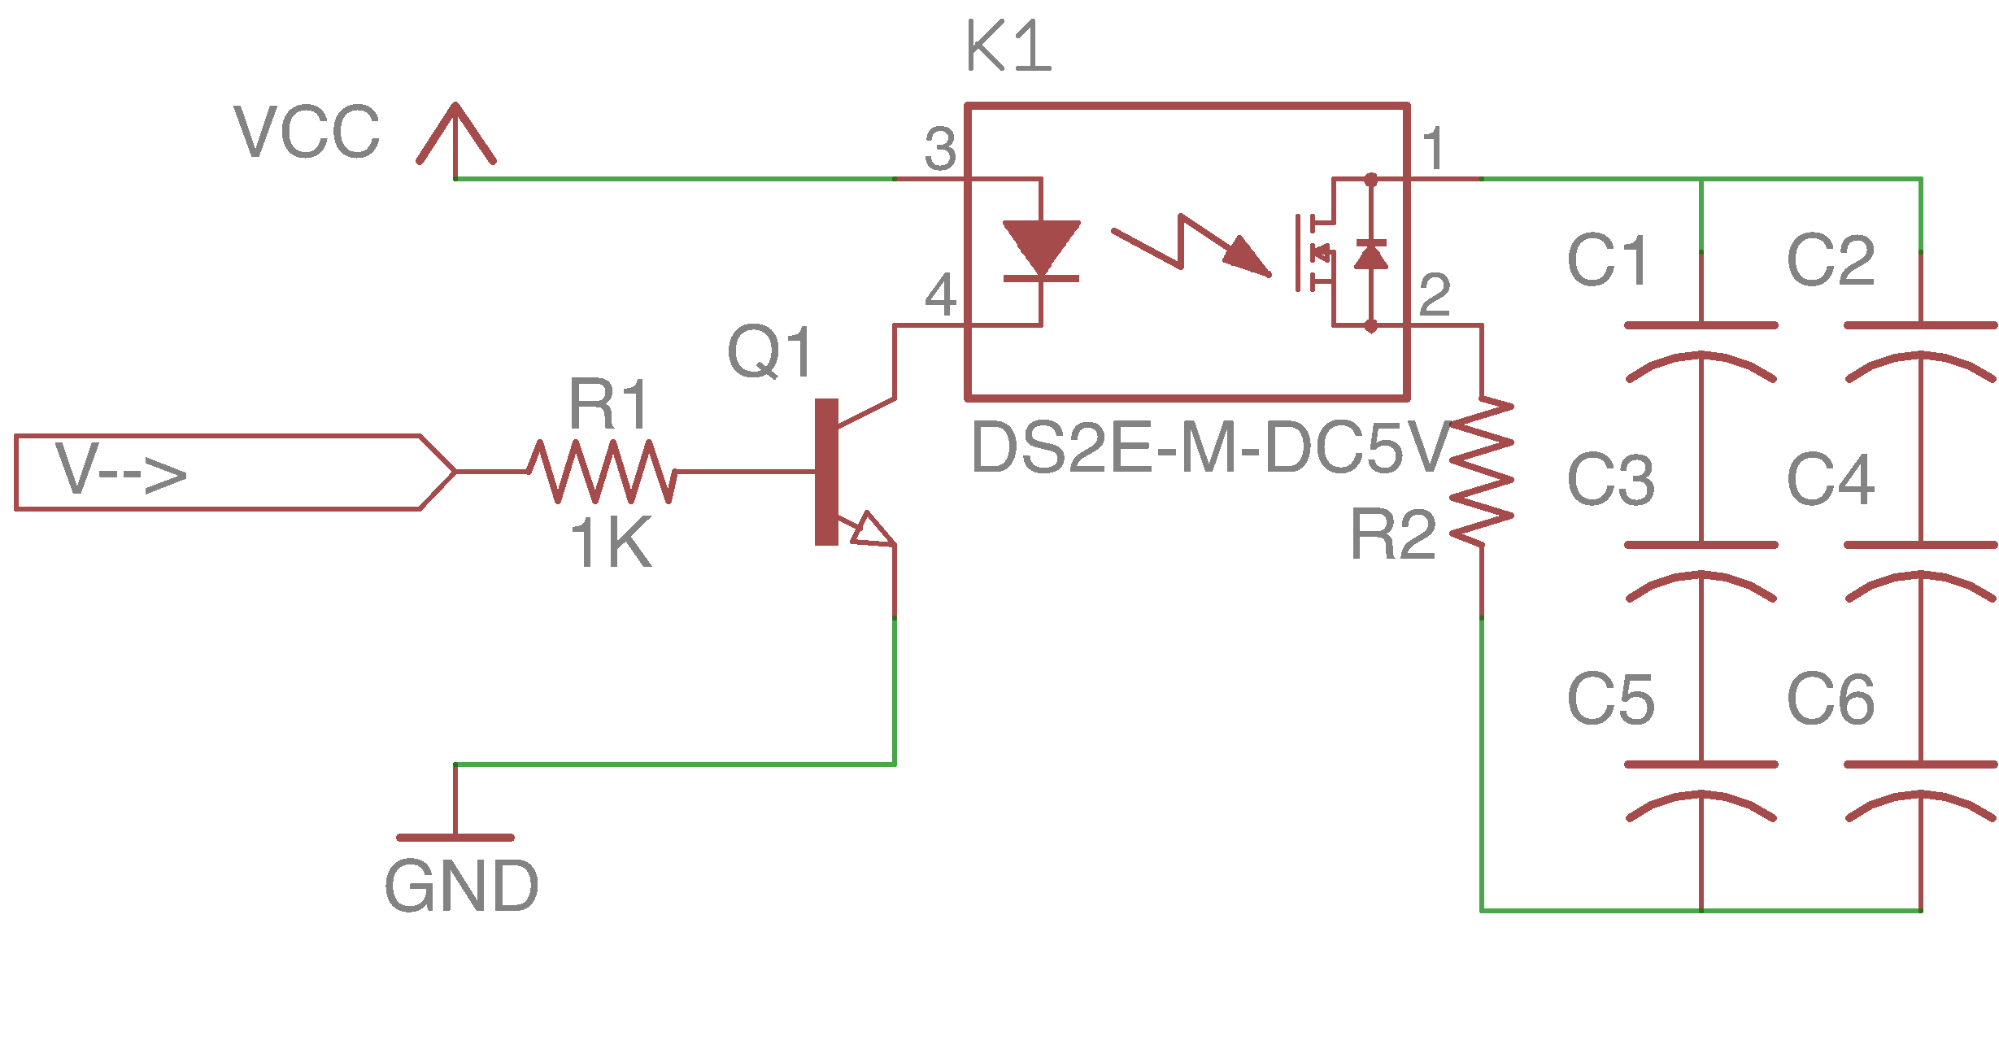
\includegraphics{assets/cutdown} 

}

\caption{\label{fig:figs} Cutdown mechanism circuit design}\label{fig:cutdown_diagram}
\end{figure}

\subsection{Cutdown Method}\label{cutdown-method}

The cutdown mechanism functions by running electricity through nichrome
wire in order to burn the string that attaches the payload to the
balloon. Two 5 cm lengths of 26g nichrome wire were used. 5 loops of the
double stranded nichrome wire were wrapped around the the string that is
to be cut. \(R_{2}\) represents the nichrome wire.

\subsection{Charge Needed}\label{charge-needed}

A stand with a 1.4 kg weight attached (the expected maximum weight of
the payload) was used as a testing apparatus. First, a power supply was
used to test the cutdown mechanism. The apparatus was placed in a
-47\degree C freezer for 30 minutes before testing. We chose this
temperature because it is colder than the expected minimum temperature
that the payload will experience. After 30 minutes, we observed that it
took 6.6A for 0.71s in order to cut the string. We calculated the amount
of charge needed to cut the string.

\[I=\frac{\Delta Q}{\Delta t}\]

The amount of charge needed is 4.7C.

\subsection{Capacitor Bank}\label{capacitor-bank}

While this is the minimum amount of charge required for the cutdown to
work, significantly more charge was stored in order to combat leaky
capacitors and cold temperatures. Our capacitor bank is composed of
supercapacitors (\(C_{1}-C_{6}\)). Each capacitor stores Three
capacitors were wired up in series. This increased the voltage of the
capacitor bank threefold. We chose to increase the voltage in order to
combat the cold conditions of space that are not favorable to the
cutdown method of heating. Electrolytic capacitors lose voltage in cold
conditions. The max voltage of the capacitor bank is calculated below.

\[V_{T} = 3V_{C}\]

The voltage of the capacitor bank is 8.1V.

Putting capacitors in series reduces their capacitance. Thus, we added
three capacitors in parallel to the original three capacitors in order
to increase the capacitance. Thus, more charge could be stored. The
capacitance of the capacitor bank (C1-C6) is calculated below.

\[C_{T} = \frac{1}{\frac{1}{C_{1}} + \frac{1}{C_{3}} + \frac{1}{C_{5}}}+\frac{1}{\frac{1}{C_{2}} + \frac{1}{C_{4}} + \frac{1}{C_{6}}}\]
The capacitance of the capacitor bank is 16.7C. The total charge stored
in this capacitor bank if it were charged at 8.1V is calculated below.

\[V=\frac{Q}{C}\]

The total charge stored is 135C. This is significantly more than the
charge needed for the cutdown to work (4.7C). Although excessive, this
ensures that the cutdown will have enough charge to function.

\subsection{Transistor Relay System}\label{transistor-relay-system}

The cutdown circuit has two power sources. VCC is the constant voltage
source supplied by the arduino. V--\textgreater{} is the cutdown signal
outputted from the arduino. Both voltage sources are 5V. Q1 is a NPN
transistor. NPN transistors work by letting current flow from the
collector to the emitter when there is a voltage applied at the base. We
used a TIP31C NPN transistor. The TIP31C requires between 1.8V and 5V of
current at the base to go on. We used a resistor between the arduino and
transistor in order to draw enough current for the base of the
transistor. When the transistor turns on, the arduinos constant 5 volt
source can send current through the switching section of a relay (K1).
When the relay is turned on, the capacitor bank (C1 - C6) can discharge
through the nichrome wire (R2).

There are two reasons for using of both a transistor and a relay. First,
transistors tend to burn out more readily when their maximum collector
current is exceeded than when a relay's maximum carrying current is
exceeded. Both the relay we used and the transistor have a maximum
current allowance of 3A. The discharging of the capacitor bank releases
a very high current. The discharge section of the circuit would benefit
from running through a component that could handle more current before
breaking. This is why a relay was used for the cutdown discharge and not
a transistor. Additionally, the relay needs to collect more current to
go on than the transistor does. Arduino signals cannot supply the needed
current to power the magnetic coils of the relay. Thus, a transistor was
used.

\subsection{Circuit Walkthrough and Physical
Design}\label{circuit-walkthrough-and-physical-design}

First, the V--\textgreater{} sends a signal that goes over R1 and into
the base of Q1. Q1 is now on and current can flow from Vcc, through the
K1 collector, through the collector and emitter of Q1, and to GND. The
relay is now on. C1-6 can discharge over R2. R2 becomes hot and cuts the
circuit.

The circuit was soldered on a lightweight protoboard. Electrical tape
was used to wrap the entire mechanism. This way, the protoboard would
not come in contact with other components in the payload and cause a
short circuit. Refer to appendix for diagrams of the cutdown mechanism
design and more physical specifications.

\subsection{Cutdown Testing}\label{cutdown-testing}

Many tests were conducted where power supplies simulated the voltage
outputs of an arduino. Over five tests conducted in this manner were
shown to cut 1.4 kg weights down at room temperature. The cutdown was
left at 38\degree C for 1 hour and 9 minutes. The cutdown still worked
in these conditions.

Next, the cutdown was tested during the tethered launch. A helium
balloon was attached at the top of the payload. The cutdown went off
while the payload was still on the ground. Pressure sensor fluctuations
were so severe that they managed to drop below the specified cutdown
pressure. To correct for this, the arduino now tests for the average of
10 readings dropping below the cutdown pressure and not single
measurements. Thus, fluctuations will be averaged out and the pressure
sensor will not incorrectly trigger the cutdown.

The cutdown was tested on a seperate arduino in a vacuum chamber. The
code used for this test follows the averaging method described above and
can be found in the appendix. The cutdown successfully burnt through a
string to release a 1.4 kg weight when the vacuum chamber dropped below
1.08 kPa. 1.08 kPa is the cutdown pressure specified in the code. This
value was chosen because it was the pressure at 100,000 ft.

\subsection{Final Code}\label{final-code}

The pressure testing cutdown code was implement into the main arduino's
code. The cutdown trigger relies on more than just the pressure in the
final code. As safety mechanisms to ensure the cutdown doesn't go off
too early, the code tests for temperature and time also. The balloon is
expected to take longer than 1.5 hours before reaching 100,000 ft.
Therefore, the cutdown will not trigger until 1.5 hours have passed.
Additionally, the temperature of the atmosphere is less than
-10\degree C at 100,000 ft. Thus, the code will not let the cutdown
trigger unless the outside temperature readings are less than
-10\degree C. The code ensures that the pressure average reading, the
temperature reading and the time all fall in the cutdown parameters for
10 readings before triggering the cutdown. This prevents from faulty
cutdown triggers due to sensor fluctuations.

There are limitations to the code that prevents the cutdown from
triggering too early. If the timer or pressure and temperature sensors
fail, the cutdown might never go off. While this error was not
encountered because the balloon popped too early (see section 8), this
was a possibility.

\section{Electrical and Software
Design}\label{electrical-and-software-design}

\subsection{Background}\label{background-1}

A circuit is a set of electronic components that are connected by wires
that conduct electricity. Electricity moves through a circuit in the
form of charge, and the measurement of the amount of charge (in
coulombs) flowing through a circuit per second is called an ampere, or
amp. A power source provides a potential energy expressed in volts,
which is a relative measure of the electric potential difference across
two nodes. These nodes are often expressed as (+), with voltage, and
(-), which is generally at 0 volts. The node with zero volts is often
called the ground (GND) because in a power supply it is often connected
to the earth, providing a reference point which can be considered at 0V.
Electricity wants to move to where there is less voltage, so when these
two sides are connected by conductive wires, the current will flow from
the positive end to the negative end. When components are connected in
series with this flow, they will receive current. The potential
difference expressed in Volts is dissipated in a circuit through a load
that takes power. In simple circuits, this can be considered a resistor.
The Voltage potential dissipated by a load with resistance \(r\) can be
related to the current across the resistance with ohm's law: \(V=IR\).
The power law states that the power dissipated by an electronic
component in Watts can be found with \(P=IV\), so therefore a component
connected in series with a circuit with current \(I\) dissipated through
resistance \(r\) is \(P=I^2R\).

A simple circuit is one where an LED is connected in the middle of the
current, which will light up the LED. However, the full voltage over an
LED with low resistance would provide too much current for the LED to
handle, so the voltage needs to be lowered, which is what a resistor
does. Resistors reduce current flow by providing electrical resistance
and dissipating power and therefore voltage in the form of heat and are
used to control the amount of voltage that reach electrical components.

\begin{figure}[h]

{\centering 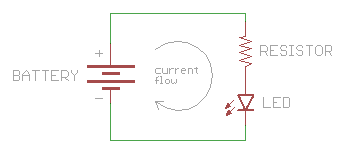
\includegraphics{assets/simple_circuit} 

}

\caption{\label{fig:figs} A simple example circuit}\label{fig:simple_circuit}
\end{figure}

Arduino is a software and hardware company that produces a variety of
microcontrollers called Arduinos that can be programmed. The Arduinos
can interact with buttons, lights, motors, the internet, and much more.
The microcontrollers have a built-in clock, memory, and voltage
regulator. The arduino operates based on the code that is uploaded to it
through the Arduino software environment, which provides an development
environment to program the arduino using C++ with special arduino
libraries built in, and a custom compiler. The way that the arduino
works with different components is through pins. These pins can serve
either to read input or as output. The first type of pins are those that
deal with power, with the Arduino having both pins that output voltage
(+) and that ground the circuit (-). Another type of pins are analog
pins, which read in a signal from an analog sensor and convert that into
a digital value. Conversely, digital pins can read input from digital
sensors, but can also output power like to an LED. There are multiple
ways to communicate with the Arduino. One way is Serial, which uses
universal asynchronous receiver/transmitter (UART) circuitry. Serial
UART is asynchronous and does not use the built in Arduino clock for
data transfer, which reduces the number of wires and pins needed to
communicate. This is how the arduino communicates with the computer
programming it, for example. Another method of communication is called
\(I^2C\) communication which uses two pins on the arduino called SDA and
SCL. \(I^2C\) communication allows for multiple ``slave'' chips to
communication with multiple ``masters'' which in our case are Arduinos.

\subsection{Electrical Design}\label{electrical-design}

The circuit consists of two Arduinos, one Mega ATK and one Uno. The Mega
ATK is our primary microcontroller and controls the logger, transmitter,
and receives input from every sensor except for the accelerometer. The
accelerometer and another microSD logger are the only two components on
the secondary Arduino Uno. The reason for the accelerometer needing it's
own Arduino is because the \(I^2C\) library it required was not
compatible with the other devices running on \(I^2C\), such as the
BME280 and spectrometer. The primary Arduino is powered by three
batteries, and one battery powers the secondary arduino and the methane
sensor. The methane sensor uses a large amount of power so it is with
the secondary Arduino's power supply so that if the sensor uses too much
power it will not disrupt the majority of the data collection and
sensors. All batteries go through 1 Amp 5 Volt voltage regulators, one
for the primary Arduino and one for the secondary Arduino and methane
sensor. The built in voltage regulator on the Arduino was not powerful
enough and causing the sensors to malfunction so exterior regulators
were included. Every sensor connects individually to either an analog
pin or digital pin, or is one of the three sensors that connect to the
SDA and SCL pins.

\subsection{Software Design}\label{software-design}

\begin{figure}[h]

{\centering 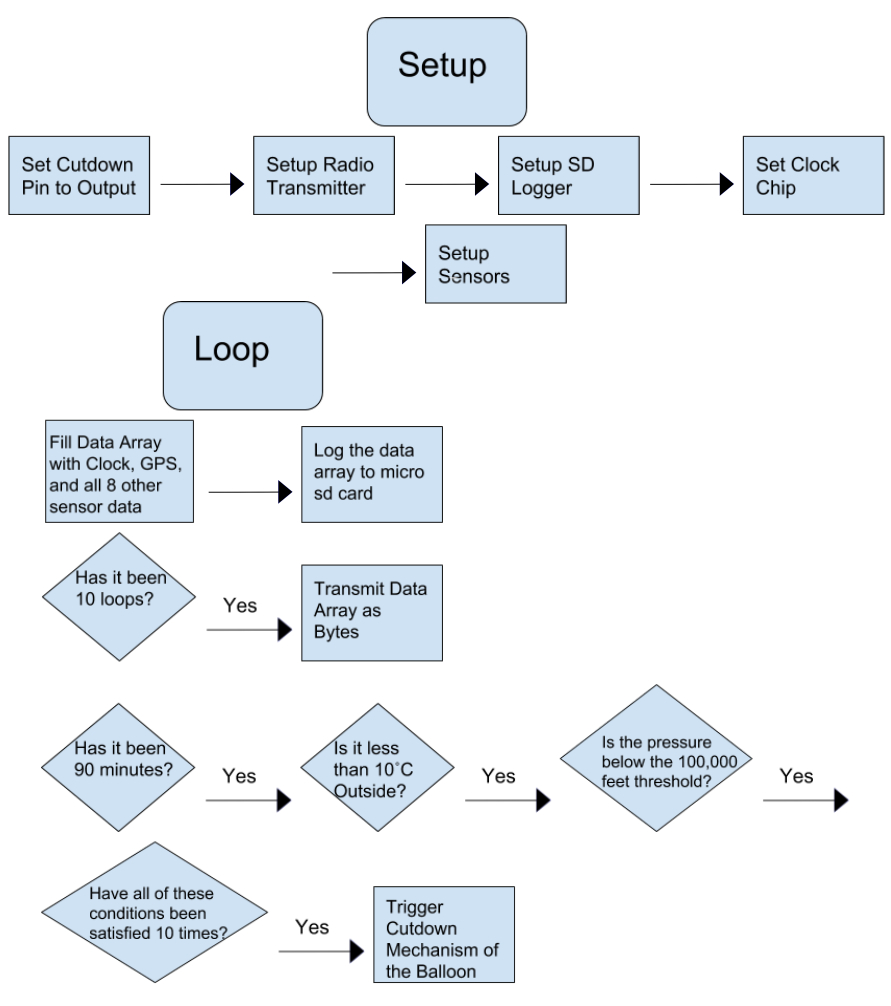
\includegraphics[height=400px]{assets/flow_code} 

}

\caption{\label{fig:figs} Code Flow Chart}\label{fig:code_flow_chart}
\end{figure}

The data acquisition organization for the microcontroller consists of
the main arduino .ino file calling methods in different header files to
get data for an array. Every loop, the data array is filled with the
current time, GPS coordinates, pressure, and more sensor data (See
Appendix V for full data index). The sensors are grouped into three
header files, one for the four individual experiments using analog
sensors, one for the BME280 exterior humidity and temperature sensor,
and one for the clock, GPS, interior temperature, and pressure sensors.
The GPS sensor uses Serial UART to send the coordinates of the antenna.
Additionally, all of the getter methods for sensors like GPS check to
make sure that if the sensor fails, the method will still return a value
so that the Arduino can continue to get the rest of the data.

Once the data array is filled, it is then logged to a microSD card by
calling a method the the sd\_logger.h file. While the data is logged
every loop, the data is transmitted down every ten loops. The radio
transmission is a large power draw and would cause some of the sensors
to be unable to receive their full voltage needed to get accurate
results, which was solved by limiting the number of transmissions to
once every ten loops.

Additionally, the accelerometer on the separate Arduino Uno logged data
constantly to its own microSD card. Since the accelerometer was not
connected to the Arduino Mega, it could not be transmitted down with the
rest of the data. The Accelerometer also logged the time since the
program had started with the built in Arduino clock. Logging the time
elapsed made it possible for the data to be matched up with the main
Arduino data using the time it logged from the exterior clock chip, and
matching that time with the start time of the secondary arduino.

\section{Tracking the Payload}\label{tracking-the-payload}

One of the largest priorities was tracking the balloon to ensure a
successful recovery. To do this, two completely independent tracking
systems were implemented to add redundancy and mitigate the chances of
completely losing the payload upon landing. The first method was a
pre-built PicoAPRS transceiver, a small separately powered 144.39 MHz
transceiver that utilizes an amateur radio network to broadcast location
details that can be accessed through a website. The backup system was
transmitting location data obtained by a Venus GPS module through a
line-of-site, point to point, 900Mhz receiver, with a novel protocol
developed with an emphasis on simplicity of parsing even broken packets.
Lastly, to narrow down the location of the payload once it touched down,
a separate transmitter at 147.065 MHz was included to use for
fox-hunting upon touchdown.

\subsection{The Global Positioning
System}\label{the-global-positioning-system}

The Global Positioning System (GPS) is a system of satellites in Medium
Earth Orbit around Earth which provide accurate location details to any
device connecting to the network. The orbits of these 31 satellites,
while not geostationary, ensure that four satellites are visible from
any location on Earth at any given moment (``GPS Systems,'' 2018). By
evaluating the time taken for GPS signals to be sent down to earth in
the form of radio waves traveling at the speed of light, a GPS receiver
is able to calculate the distance between it and the satellite. Using
this distance information gained from at least three satellites, a GPS
receiver is then able to ``trilaterate'' to find its location relative
to the satellites (``How Does,'' n.d.). Given the distance between a
satellite, a GPS unit must be located on a sphere extending outward with
a radius of that distance. With information from three satellites, three
spheres are given, and generally the intersection of three spheres
results in two points, once which can be discarded due to the fact that
it would not be physically possible for the GPS receiver to be located
there.

The Department of Commerce has placed regulations on exports that could
potentially threaten the United States. This includes GPS receivers that
can provide data when they are above 18,000 meters or their speed is
above 1000 knots, due to their potential use in Intercontinental
Ballistic Missiles (COCOM GPS Tracking, n.d.). Some manufacturers have
implemented these limits by shutting down the system when either
condition is met, and some manufacturers have implemented these limits
by shutting down the system only if both conditions are met. This is an
important distinction, since high altitude balloons often exceed the
height limit of 18,000 meters. Sparkfun's Venus GPS module, which uses
the Venus634FLPx GPS chipset, is known to allow altitudes of over 18,000
meters, given that the speed of the GPS receiver is not calculated to be
more than 1000 knots (GPS Modules, 2016).

\subsection{The PicoAPRS Transceiver}\label{the-picoaprs-transceiver}

The primary tracking system onboard the balloon was a PicoAPRS,
developed by Taner Schenker (DB1NTO). This is a small transceiver that
can receive and broadcast on the Automatic Packet Reporting System
(APRS). Most importantly, it contains its own separate GPS chip that
allows it to broadcast its location to the APRS network. This device is
completely self contained, including its own 850MAh Lithium Ion battery,
making it a perfect candidate for tracking -- even if all other systems
on the balloon have failed, the PicoAPRS should still be able to
transmit its location. Furthermore, the PicoAPRS provides a simple menu
for device configuration, to enable the performance desired.
Specifically, the PicoAPRS transmitted GPS beacons at a power of 1 Watt
over intervals of 60 seconds. The PicoAPRS did this with Menlo School's
callsign, N6MLO, and a unique SSID, 9, that differentiated the packets
sent by 6thsense's PicoAPRS from other concurrent Menlo School balloon
launches.

\subsection{The APRS Network and
MIC-Encoding}\label{the-aprs-network-and-mic-encoding}

A very important benefit of using the PicoAPRS is that it uses the
Automatic Packet Reporting System (APRS). This amateur radio network,
developed by Bob Bruninga (WB4APR) uses digipeaters to forward properly
formatted broadcasted beacon packets to other stations in the area to
effectively extend the range of a single transmitter (Bruninga, n.d.).
Rather than focusing on ensuring that a packet is received by all
digipeaters, this protocol focuses on redundancy through packet
``multiplication'' by having each digipeater that receives the signal
propagate it outward through the network. While the exact details of how
many ``hops'' a packet can take through the network before transmission
ends are dependent on the settings present in the header of the packet.
This system became popular, especially for transmitting GPS data and
tracking vehicles, and eventually specifications were developed to
transfer packet data to the web through APRS-Internet Service (APRS-IS)
(Loveall, n.d.). The aprs.fi website, which interfaces with APRS-IS and
displays live telemetry data superimposed on google maps, provided a
simple method of tracking the balloon during the launch.

The APRS network transmits packets through a single AX.25 data link
protocol, which specifies the structure of frames to be sent through the
network (Buthod, 1997). Specifically, it uses Unnumbered Information
(UI) frames, a type of AX.25 frame that is transmitted without any
expectation of a response confirming reception, and reception is not
guaranteed. APRS supports different encoding of these AX.25 UI-frames,
however, to allow for different uses of the network. The PicoAPRS
transmitter uses ``Mic-Encoding'' (MIC-E), a method that allows for
extremely compressed packets that still contain position, course, speed,
a message, and all relevant path settings and necessary headers
(Bruninga, n.d.). This achieved by writing compressed latitude
information in the destination address field of the AX.25 frame, and
compressed Longitude information in the frame's Information Field (Wade,
2000). By transmitting extremely short packets that are still supported
by the APRS network and aprs.fi, Mic-E can improve the reliability of
the beacons transmitted.

APRS is transmitted using Frequency Modulated signal at 144.39 MHz.
Frequency Modulation works by altering the frequency of a carrier wave
to encode information.

The PicoAPRS was chosen because the system had worked historically for
past ASR Balloon Launches. During testing, however, the APRS network
often failed to receive beacons, due to the fact that most tests were
conducted at ground level, where line of sight to repeater stations was
often not available. Furthermore, there was no method of testing the
maximum altitude that beacons could be sent from before connection to
the APRS network was lost. Lastly, since Lithium-Ion batteries are known
to work poorly in below freezing temperatures, there were concerns that
the unit might shut down once the temperature dropped, if not properly
insulated. Due to these concerns, a backup tracking system was developed
that did not rely on the PicoAPRS and APRS network should the PicoAPRS
unit fail.

\subsection{The 900MHz Venus GPS
Transciever}\label{the-900mhz-venus-gps-transciever}

The backup tracking system involved sending GPS along with other
telemetry data from the main arduino mega to the base station using
Digikey 9XTend 900MHz transceivers (9XTend OEM RF Module, n.d.). The use
of these transceivers provided a high power 1 Watt signal in a
relatively clear band that let a novel communications protocol be
implemented that allowed for ease of parsing. The 9XTend module
interfaced easily with both balloon and base station arduinos through
Universal Asynchronous Receiver-Transmitter (UART) Serial. Since the
Arduino Mega provides three usable Serial ports, one was used to send
data to the 9XTend Module. By taking advantage of Arduino's Serial
library, a library was developed that allowed the 9XTend modules to
transmit ASCII encoded bytes, which, given some stream editing by the
base station to remove ASCII control characters injected by the base
9XTend Module, is parsable as an ASCII byte stream by software on the
base station.

\subsubsection{A Novel Transmission
Protocol}\label{a-novel-transmission-protocol}

To send readable GPS and telemetry data to the base station, a simple
multi-layer protocol was implemented with design considerations in mind
to allow for simple parsing and data analysis, simple manual error
detection, no error correction or discarding of broken transmissions, no
set packet size, zero unnecessary headers or other packet configuration
information, and no transmitter handshaking requirements. This allows
for simplex communication between the payload and base station. This
also ensures that all bytes that are received by the 9XTend, which
implements a Cyclic Redundancy Check on every byte received to ensure
its value is correct, are sent to the base station software for parsing.
Note that the 9XTend module not protect against lost bytes, so packets
could often be broken or missing some information. Through this new
protocol, no partially broken packets would be lost or deleted if the
signal was weak. Since the 9XTend Module transmitted all data for
sensors connected to the arduino as a redundancy in case the payload was
not retrieved or there was a problem logging data to the onboard SD
card, it is also crucial to be able to differentiate between two
different values in a partially broken packet.

A protocol was used with the following form to transmit n values:

\texttt{******\textless{}value-1\textgreater{}-\/-\/-\/-\/-\/-\textless{}value-2\textgreater{}-\/-\/-\/-\/-\/-...-\/-\/-\/-\/-\/-\textless{}value-n\textgreater{}}

Where \texttt{\textless{}value-i\textgreater{}} is an ASCII encoded,
calibrated and human readable sensor value. This allows for simplex
operation in which a base station can tune in at any time--if the base
station loses reception or power for some reason, it can listen in for
the next packet when it comes back online by simply waiting for the 6
stars indicating the start of a packet. Furthermore, data was encoded in
ASCII bytes to let the output be human readable with little computation.
This way, the output stream could be easily analyzed without having to
convert bytes containing raw numerical values into ASCII text. This gets
rid of the need to make specifications for negative numbers and floats,
and the need to specify the size of transmitted data. By encoding each
digit as an ASCII byte, it was simple to account for negative numbers by
preceding the value with a dash just as is normally done with displayed
numbers, and to account for floats by adding a decimal place behind the
ones digit. Furthermore, more complicated sensor readings like GPS and
Spectrometer output that contained ASCII formatted text could be sent
as-is with zero need for manipulation. Since 12 values were transmitted
(refer to Section 5) with uncompressed ASCII bytes, packet sizes were
long: up to 240 bytes. Because of this, there were often small failures
in the packet were a byte or series of bytes was not received. Such
packets were still logged with the notion that it was still possible to
extract most of the data out of them instead of having them completely
go to waste. To ensure that the start of a packet could be recognized
and separate values could be delineated properly, however, a full six
bytes was used to mark the beginning of a transmission, and breaks
separating values. This data was only transmitted about once every 12
seconds, partly to serve as flow control in order to not overload the
transmitter's buffer, and partly to conserve battery power, as the
9XTend module consumed 1 Watt while transmitting and was connected to
the same battery as the Arduino Mega running all the sensors and SD
logger.

\subsubsection{Physical Considerations and Antenna
Design}\label{physical-considerations-and-antenna-design}

Since the 9XTend module transmits directly to the base station, line of
sight was crucial to maintain connectivity. An omnidirectional whip
antenna had to be used on the balloon module since the heading and
position relative to the base station was constantly changing and
therefore the transmissions could not be directed in one particular
direction. While it might have been possible to use a directional
antenna at the base station to increase signal, it was not ideal since
the balloon was followed in a chase van, and directing an antenna
outside the van would be imprecise and lead to a lossy connection.
Furthermore, 900MHz yagi antennas are not readily available in stores
and time was not properly budgeted to assemble and test one by hand.
Therefore, a 900Mhz whip antenna was mounted to the top of the chase van
to connect to the receiving 9XTend Module.

\subsection{Fox-Hunting with a 147.065MHz
Transmitter}\label{fox-hunting-with-a-147.065mhz-transmitter}

While GPS modules, if they have signal at ground level, are usually able
to report location down to a few feet, the PicoAPRS was only expected to
be able to connect to the APRS network at a few thousand feet before it
lost line of sight to repeater stations, and there was no expectation to
receive signal from the 900MHz point to point transmitter, which also
relied on line of sight, which would not be available when the payload
had touched down. Therefore, it was expected that the latitude and
longitude data provided by both the PicoAPRS and the 9XTend modules
would be too imprecise to be able to locate and retrieve the payload. To
further narrow down the location of the module, a 147.065MHz transmitter
was included that broadcasted a distinct audio beacon along with Menlo
School's callsign in morse code, every minute. This enabled the use of
Fox-Hunting techniques to recover the payload once the tracking team was
in range of the beacon.

By having an omnidirectional whip antenna transmit the beacon and a
directional yagi antenna receive the beacon, the direction of the
balloon relative to the fox-hunt receiver was able to be calculated once
the fox-hunt receiver was in range of the beacon. Since directional
antennas receive greater power in the direction they're pointed, by
identifying in which direction the antenna receives the strongest
signal, it is possible to identify the source of the beacon and move in
that direction until the payload is found.

\subsubsection{Fox-Hunting Yagi Antenna
Design}\label{fox-hunting-yagi-antenna-design}

For Fox-Hunting, a 3 element yagi antenna was built with the appropriate
lengths and spacing to receive signals at around 147.065mHz (see section
3). It provides approximately 7.2db of forward gain. The 3 element yagi
is the most basic arrangement, with a single director, driven element,
and reflector. The driven element is a dipole which receives the
incoming signals and transmits it to the radio. The unique
directionality of the yagi is a result of the reflector element and
director element working together to shape and amplify the range of the
beam in a particular direction (``Yagi Antenna,'' n.d.).

\subsubsection{Determining Signal Strength with a Variable RF
Attenuator}\label{determining-signal-strength-with-a-variable-rf-attenuator}

A crucial component of Fox-Hunting is measuring the received signal
strength. Since the transmitter transmits an audio signal, one can
simply listen to the clarity of the received audio to do so. If the
receiver is close to the transmitter, however, and the received signal
is very strong, in tests it was hard to differentiate between a weak and
a strong signal and narrow down on the proper direction. To be able to
better distinguish signal strength, a variable Radio Frequency (RF)
attenuator was used to lower the strength of the signal until distortion
in the audio could clearly be heard, and therefore it was easier to
determine whether the signal strength improved or decreased after a
change in direction of the antenna.

The RF Attenuator used to lower the received signal mixes a constant
4MHz with the received signal in order generate two sidebands 4MHz above
and below the base signal. This sideband is an attenuated version of the
original signal, and tuning the receiving radio to the base frequency
plus 4 MHz, 151.065MHz, lets one monitor this attenuated signal.
Furthermore, the amplitude of the 4 Mhz signal can be varied in order to
vary the strength of the sideband, effectively providing varied
attenuation.

\subsection{Results}\label{results}

The balloon powered on at precisely 1:00pm with all three systems
working: location information showed up on aprs.fi, the base station
received transmissions including GPS information, and the HAM radio used
for fox-hunting received 6thsense's unique tone.

\subsubsection{The Venus GPS and 9XTend
Module}\label{the-venus-gps-and-9xtend-module}

Only about 14 minutes later, however, once the balloon had reached
approximately 2600 meters, the Venus GPS module lost reception and
stopped transmitting latitude and longitude data. The 9XTend module
continued to transmit other telemetry data including altitude, however,
for the duration of the flight, until the payload touched down, in which
most likely the crash disconnected some circuitry essential to
transmission, or the batteries lost their charge. Once the payload
reached approximately 7800 meters, 9XTend transmissions became
significantly damaged to the point where the data could no longer be
programmatically parsed by simply finding values between the delimiters
specified. Packets continued to be somewhat recognizable up to 20,000
meters, the estimated maximum height the ballon reached at approximately
1:50pm. Shortly after, at 1:53pm, the first packet was received
indicating the balloon had began a slow descent (discussed in detail in
section 8). During descent, especially back at around 7800 meters,
transmissions became more recognizable but still required manual
interpretation. Transmission stopped after around 7400 meters,
indicating that most likely the arduino lost power at 2:17pm, two and a
quarter hours after powering up. The density of packets received from
the 9XTend as a function of time and altitude can be seen in in Figure
\_\_, in Section 8.

Unfortunately, while the 9Xtend module paired with the Venus GPS failed
its primary mission of providing GPS information, the transmission
system worked very well for the entirety of the time that it was
powered. Not only did it provide the base station with live altitude
data, it transmitted sensor data, including that of individual
experiments. This proved invaluable to the team, since the SD logging
module failed to write data.

Since the Venus GPS receiver was mounted at the top of the payload, with
its line of sight to the GPS satellites obstructed by only the balloon,
and the GPS chips did not have the 18,000 meter limit, there is no clear
reason for why the system failed. One possibility is that the outside
temperature of 16 degrees Celsius was too low for the circuitry
involved. Another is simply that the antenna was somehow internally
damaged or not optimal. Upon touchdown, all GPS wiring was still in
place, indicating that it was not an issue with the circuit or placement
of the antenna.

The last possible reason is that other circuitry such as the arduino
microprocessor in the payload generated radio frequency interference.
The GPS center frequency is 1575.42MHz, however, and the crystal
oscillator providing the clock for the Arduino Mega only runs at 16MHz,
which indicates that other circuits in the payload were most likely not
causing this issue.

\subsubsection{The PicoAPRS and APRS
Network}\label{the-picoaprs-and-aprs-network}

The PicoAPRS consistently broadcasted packets that were picked up by the
network up to almost exactly 10,000 meters at 1:30pm, before the network
lost reception. The PicoAPRS continued transmitting accurate location
data, however, and the network once again started receiving
transmissions at 2:16pm, once the payload had fallen to approximately
8200 meters. The final transmission came at 2:36pm just 250 meters above
the ground. Overall, this system worked flawlessly to provide accurate
location data while in range of the network, between approximately 250
meters and 9000 meters in altitude. Fortunately, the insulation added to
the payload was able to keep its Lithium Ion battery warm enough to
maintain power. Since the Venus GPS failed early into the flight,
tracking the payload relied on the APRS for accurate location data until
the chase van got in range of the fox-hunt beacon. APRS network
connectivity as a function of time and altitude can be seen in Figure
\_\_, in Section 8.

\subsubsection{The Fox-Hunt Beacon and Yagi
Antenna}\label{the-fox-hunt-beacon-and-yagi-antenna}

The final PicoAPRS beacon came from a very low altitude, narrowing down
the final location to a radius of less than 200 meters. Once the chase
van arrived at the location described by the final APRS packet, the team
was immediately able to pick up the Fox-Hunt signal even with the
attenuator attached. A single sweep of the Yagi antenna revealed the
payload was due South along the road, and the payload was found less
than 50 meters away from the road, lying hidden from view of the road on
a small hill. The antenna, attenuator, transmitter and receiver all
worked flawlessly to lead to a simple recovery in the time it took to
walk from the parked van to the touchdown point of the payload.

\section{Sensor Calibration}\label{sensor-calibration}

To ensure that the payload would collect accurate and reliable data, the
lightweight sensors used and controlled by the Arduino board were
thoroughly calibrated. The three group sensors calibrated were the
temperature and humidity sensors onboard the Vernier Gas Pressure
Sensor, and the Vernier Gas Pressure Sensor. The outputs of all three
sensors were compared to standards, which were already known to be
reliable and accurate. The standards, despite their accuracy, could not
be used in the payload because of their heavy weight and large size,
hence it was crucial that the small and light Vernier and BME280 sensors
were calibrated.

\subsection{Pressure}\label{pressure}

The Vernier Gas Pressure Sensor, model GPS-BTA, was calibrated to the
Extech SD700 Barometric Pressure/Humidity/Temperature Datalogger, which
was used as the standard for pressure. The Vernier sensor was connected
to an Arduino microcontroller with a Vernier Analog Protoboard Adaptor
and configured to log data onto a micro-SD card every 1.50 seconds.
Instead of having a output unit of hPa or kPa, the Arduino maps input
voltages between 0 to 5 volts to 10-bit integer values between 0 and
1023---a total of 1024 bins with 0.0049 V resolution. Thus, each unit
represents 4.9 mV. The SD700 has a pressure range of 10 to 1100 hPa,
fine resolution of 0.1 hPa, optimal temperature range of 0 to 50°C,
response time of 10 milliseconds, and total accuracy with its factory
calibration ±2 hPa. It requires 6 AAA batteries, and records data to an
external SD card in the format of an Excel worksheet. It was configured
so that it sampled data every five seconds to have smoother and more
gradual changes in pressure. After both sensors were turned on at the
same time to easily compare the data later, they were immediately placed
in a vacuum chamber, in which air and other gasses are removed by a
vacuum pump, thus creating a low-pressure environment inside the
chamber. The release valve was closed and the vacuum pump was opened.
When the pressure reading from the valve reached its minimum of
approximately 0 hPa, the vacuum pump was then disconnected. An important
part of the pressure calibration process was having ``plateaus,'' or
multiple data points at various pressure levels. To have plateaus in the
data, the release valve was slowly opened and closed right after, and
this process was repeated after waiting approximately 45 seconds
multiple times. Figure 5 shows the varying pressure readings from the
standard Extech sensor and Arduino Vernier sensor across time.

\begin{figure}[h]

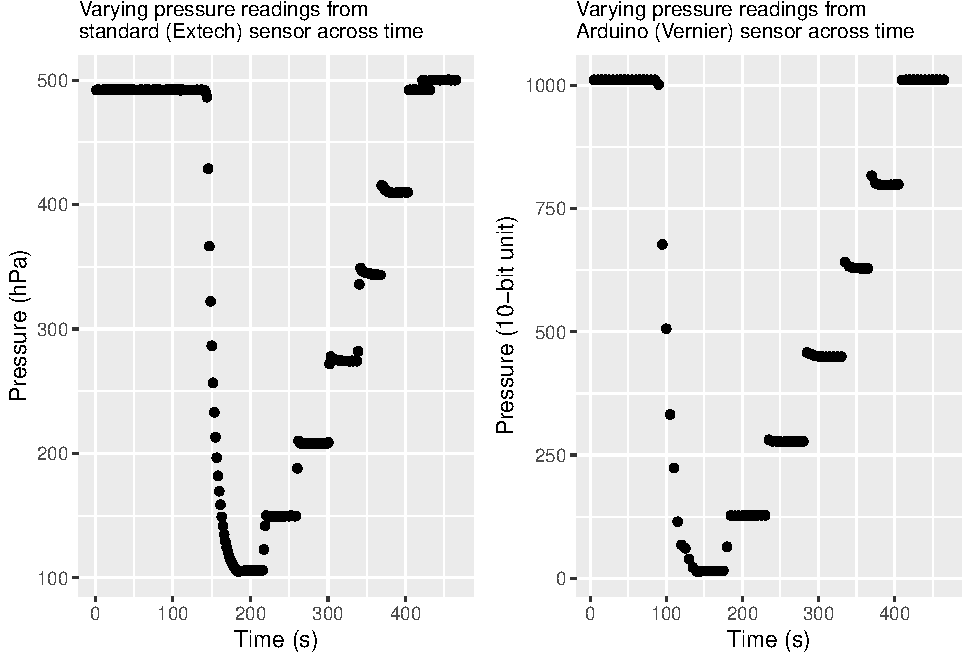
\includegraphics{paper_files/figure-latex/vernier_calibration-1} \hfill{}

\caption{\label{fig:figs}}\label{fig:vernier_calibration}
\end{figure}

Figure 6 shows the conversion between the output of the standard
(Extech) sensor and that of the Arduino (Vernier) sensor, including the
equation to convert the Arduino's 4.9 mV resolution units to kPa.

\begin{figure}[h]

{\centering 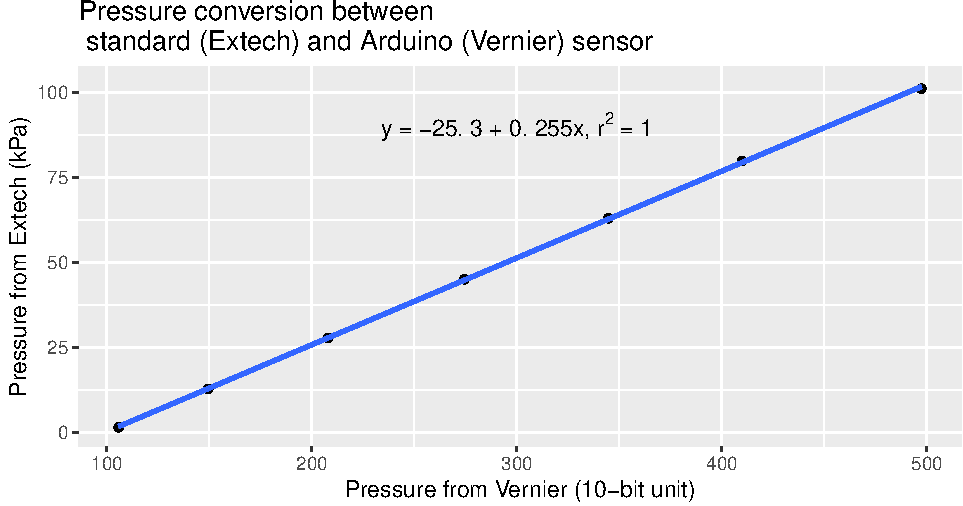
\includegraphics{paper_files/figure-latex/vernier_cal2-1} 

}

\caption{\label{fig:figs}}\label{fig:vernier_cal2}
\end{figure}

Below is example data used to calibrate the Veriner Pressure Sensor.

\begin{longtable}[]{@{}rr@{}}
\caption{Varying average pressure readings from Arduino (Vernier)
vs.~Standard (Extech) sensor}\tabularnewline
\toprule
Vernier sensor (10-bit unit) & Extech sensor (kPa)\tabularnewline
\midrule
\endfirsthead
\toprule
Vernier sensor (10-bit unit) & Extech sensor (kPa)\tabularnewline
\midrule
\endhead
105.77 & 1.48\tabularnewline
149.44 & 12.75\tabularnewline
207.92 & 27.79\tabularnewline
274.45 & 45.04\tabularnewline
344.59 & 62.95\tabularnewline
409.80 & 79.86\tabularnewline
497.34 & 101.09\tabularnewline
\bottomrule
\end{longtable}

\subsection{Humidity}\label{humidity}

The Adafruit BME280 sensor, which takes data on temperature, barometric
pressure, and humidity, was calibrated to a Vernier Relative Humidity
Sensor for humidity and the Fieldpiece ST4 Dual Temperature Meter for
temperature. The BME280 humidity sensor has an operating temperature of
-40 to 85°C, response time of 1 second, and total accuracy of ±3 \%RH.
To calibrate for humidity, the BME280 was connected to an Arduino mega
with header pins and programmed to print out data every second to the
serial monitor. The standard for humidity, a Vernier humidity probe, was
connected to the same Arduino board via the Analog Protoboard Adaptor
and also programmed to print out its humidity readings in the serial
monitor every second. The Vernier Relative Humidity Sensor has a
humidity range of 0 \% to 95 \%, resolution of 0.16\% RH, operating
temperature range of 0 to 85°C, response time of 40 seconds, and total
accuracy with its standard calibration of ±10 \%RH. Both sensors were
exposed to environments with various humidity levels: the Menlo Quad at
3:00 PM and a shower 30, 60, 90, and 120 seconds after turning the hot
water on. Multiple consecutive relative humidity readings from both
sensors at each time point were then manually recorded in a csv file.
Figure 7 depicts the relative humidity conversion between the output of
the standard (Vernier) sensor and that of the Arduino (BME280) sensor
across various humidity levels.

\begin{figure}[h]

{\centering 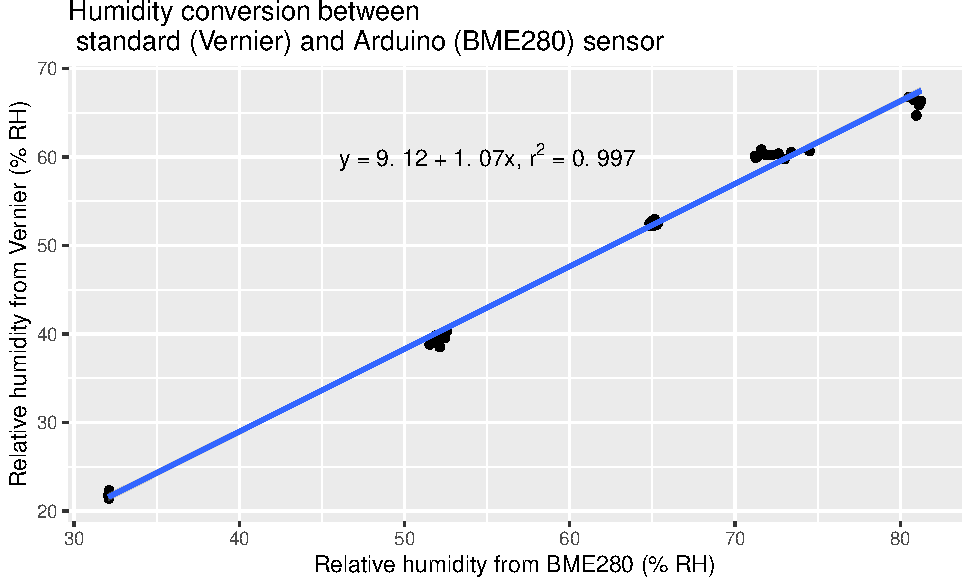
\includegraphics{paper_files/figure-latex/bme-1} 

}

\caption{\label{fig:figs}}\label{fig:bme}
\end{figure}

\section{Temperature}\label{temperature}

In order to calibrate the temperature readings of the BME280 to a
standard, the Fieldpiece ST4 Dual Temperature Meter, both sensors were
placed in multiple locations of varying temperatures: a freezer,
refrigerator, and the Menlo Quad at two different times of the day. The
BME280 sensor has an operating temperature range of -40 to 85°C,
absolute accuracy of ±1.0°C, and resolution of 0.01°C. The Fieldpiece
sensor has a functional temperature range of -50 to 1300°C, resolution
of 0.1°C, ±2°C in cold temperatures from -50 to 0°C, and sample rate of
2.5 readings every second. It takes two readings at the same time due to
the two temperature rods available, T1 and T2; however, only T1 was used
across the experiment because T2 fluctuated significantly more than T1.
Since the Fieldpiece sensor could not log data into an SD format or
connect to an external controller interface for monitoring, the only way
to calibrate the BME280 sensor to the Fieldpiece was to manually record
the two list of temperature readings displayed in the serial monitor.
Figure 8 shows the temperature conversion between the output of the
standard (Fieldpiece) sensor and that of the Arduino (BME280) sensor
across various temperatures.

\begin{figure}[h]

{\centering 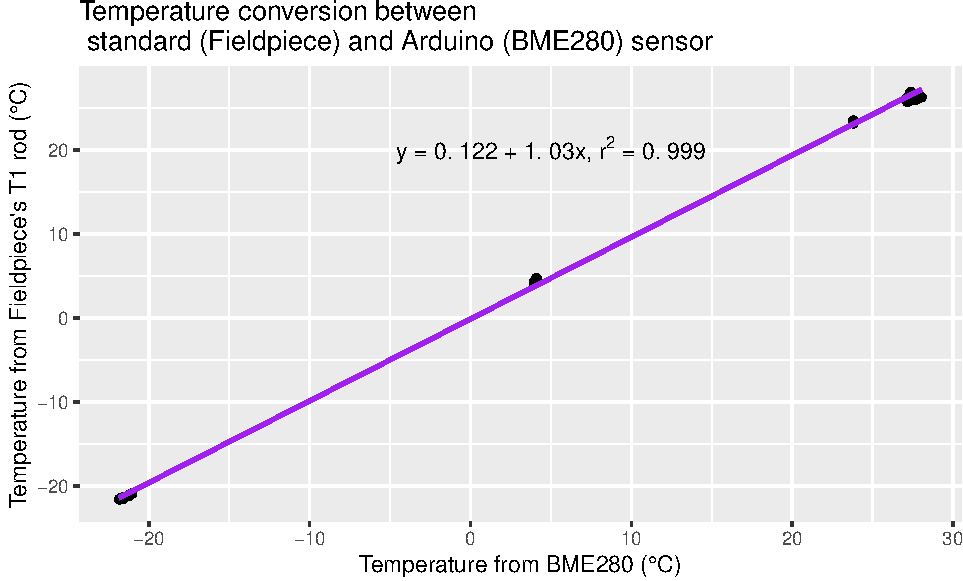
\includegraphics{paper_files/figure-latex/bme_temp-1} 

}

\caption{\label{fig:figs}}\label{fig:bme_temp}
\end{figure}

However, it was later found much after the final launch that the BME280
sensor had failed during the payload's ascent and did not transmit or
record any useful data. Thanks to a thermistor attached to the main
board as backup, the payload was still able to transmit temperature data
throughout its flight into the stratosphere. However, the thermistor was
not calibrated to a standard before the launch because the BME280 had
been expected to function properly without issues. Once the payload was
retrieved, only then could the thermistor be calibrated to the Extech
SD700, which has both an accurate pressure and temperature sensor,
resolution of 0.1°C, and accuracy of ±0.8°C. The Extech SD700 was used
as the standard instead of the Fieldpiece ST4 because the SD700 was
found to be more accurate than the previously used ST4 after the final
launch. Graph 10 below shows the temperature conversion between the
output of the standard (Extech) sensor and that of the thermistor on the
Arduino board across various temperatures. It is noted that data from
the thermistor has units of 10-bit voltage units that range from integer
values 0 to 1023, each with a resolution of 4.9 mV. These units were
converted to degrees in celsius following a equation provided by the
thermistor's manufacturer to ultimately visualize a linear regression
instead of a logarithmic curve during calibration.

\begin{figure}[h]

{\centering 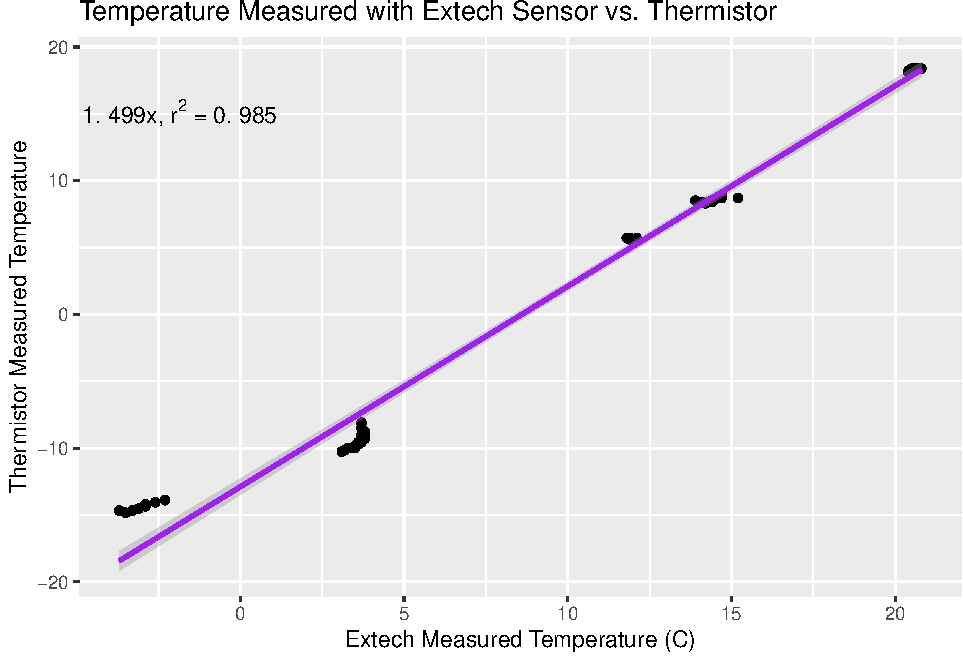
\includegraphics{paper_files/figure-latex/temp2-1} 

}

\caption{\label{fig:figs}}\label{fig:temp2}
\end{figure}

\subsection{Error Bars}\label{error-bars}

The data gathered from the pressure, humidity, and temperature sensors
do not all accurately represent the universally true values. There is
bound to be inaccuracy from at least one of the three sources of error:
accuracy, resolution, and calibration of the sensor. The standard for
pressure and temperature, the Extech SD700, has a very high accuracy of
±2 hPa and , which can be disregarded as insignificant. Using Graphical
Analysis and the LINEST function in Excel, the uncertainty of the slope
of Graph 7 was calculated. Thus, the percent error of the slope =
uncertainty of slopeslope*100, which was later multiplied with all of
the pressure readings collected by the sensor to calculate error bars.
To calculate the error bars that either contain or depend on the
humidity and temperature data, multiplying the percent error of the
slope of the conversion graphs does not work because the accuracy of the
standards could not be regarded as perfectly accurate. Instead of solely
using the percent errors, the room mean square error (RMSE) was found
for all sensors, as shown below in Table 5. Table 6 lists the total
errors and percent errors for the four main experiments---one extra due
to the addition of the thermistor calibration after the final launch.

\textbf{JOHN INSERT RMSE TABLE HERE}

\begin{longtable}[]{@{}lr@{}}
\caption{Percent errors for the group sensors used relative to
standards}\tabularnewline
\toprule
Experiments & Percent error (\%)\tabularnewline
\midrule
\endfirsthead
\toprule
Experiments & Percent error (\%)\tabularnewline
\midrule
\endhead
Pressure & 0.459\tabularnewline
Humidity & 0.659\tabularnewline
Temperature & 0.429\tabularnewline
\bottomrule
\end{longtable}

\section{Experimental Results}\label{experimental-results}

In the span of an hour and a half, the payload traveled 90 kilometers
(56 miles), and reached an estimated maximum height of approximately 20
kilometers (12 miles). APRS packets show the balloon reached speeds of
at least 111 km/h in the jet stream, and transmissions data shows the
balloon spent significant time in the ozone layer. Figure \_\_ shows the
altitude calculated with the two tracking systems on board, as a
function of time. Note that the density of the points correspond to the
connectivity of each method of data retrieval at that altitude and
moment in time.

\begin{figure}[h]

{\centering 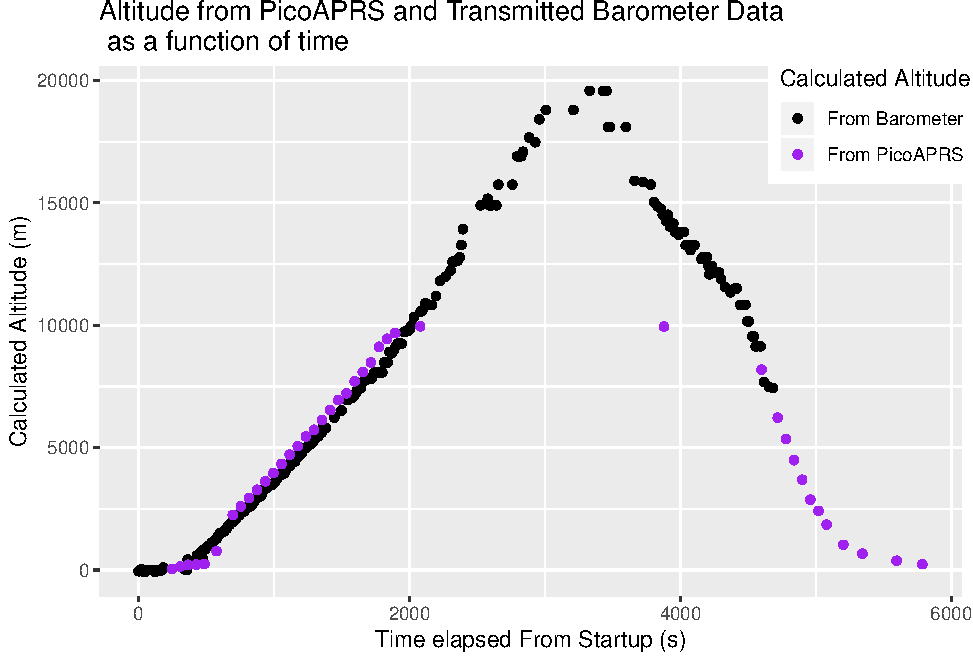
\includegraphics{paper_files/figure-latex/altitude-1} 

}

\caption{\label{fig:figs}}\label{fig:altitude}
\end{figure}

As seen in Figure 10, APRS data for the altitude lines up extremely
closely with the altitude calculated from the barometer. The small shift
is most likely due to a difference in timing: the PicoAPRS transceiver
was on a separate clock than the arduino, and it is plausible that the
timing was off by mere seconds.

\subsection{Descent}\label{descent}

The cutdown never went off because the balloon never detached from the
payload. The lowest recorded pressure sensor data was 5.86 kPa. Using
NASA's model for the relationship between pressure and altitude, this
suggests that our ballon reached a max altitude of 64222 ft. This was
below the cutdown height of 100,000 ft. The balloon began accelerating
downwards at approximately 50 minutes into the flight (refer to altitude
vs.~time graph).

Go-Pro footage reveals that the balloon was popped by our APRS antenna.
Stills from the footage (approximately 32 minutes into the flight) are
shown below.

\begin{figure}[h]

{\centering 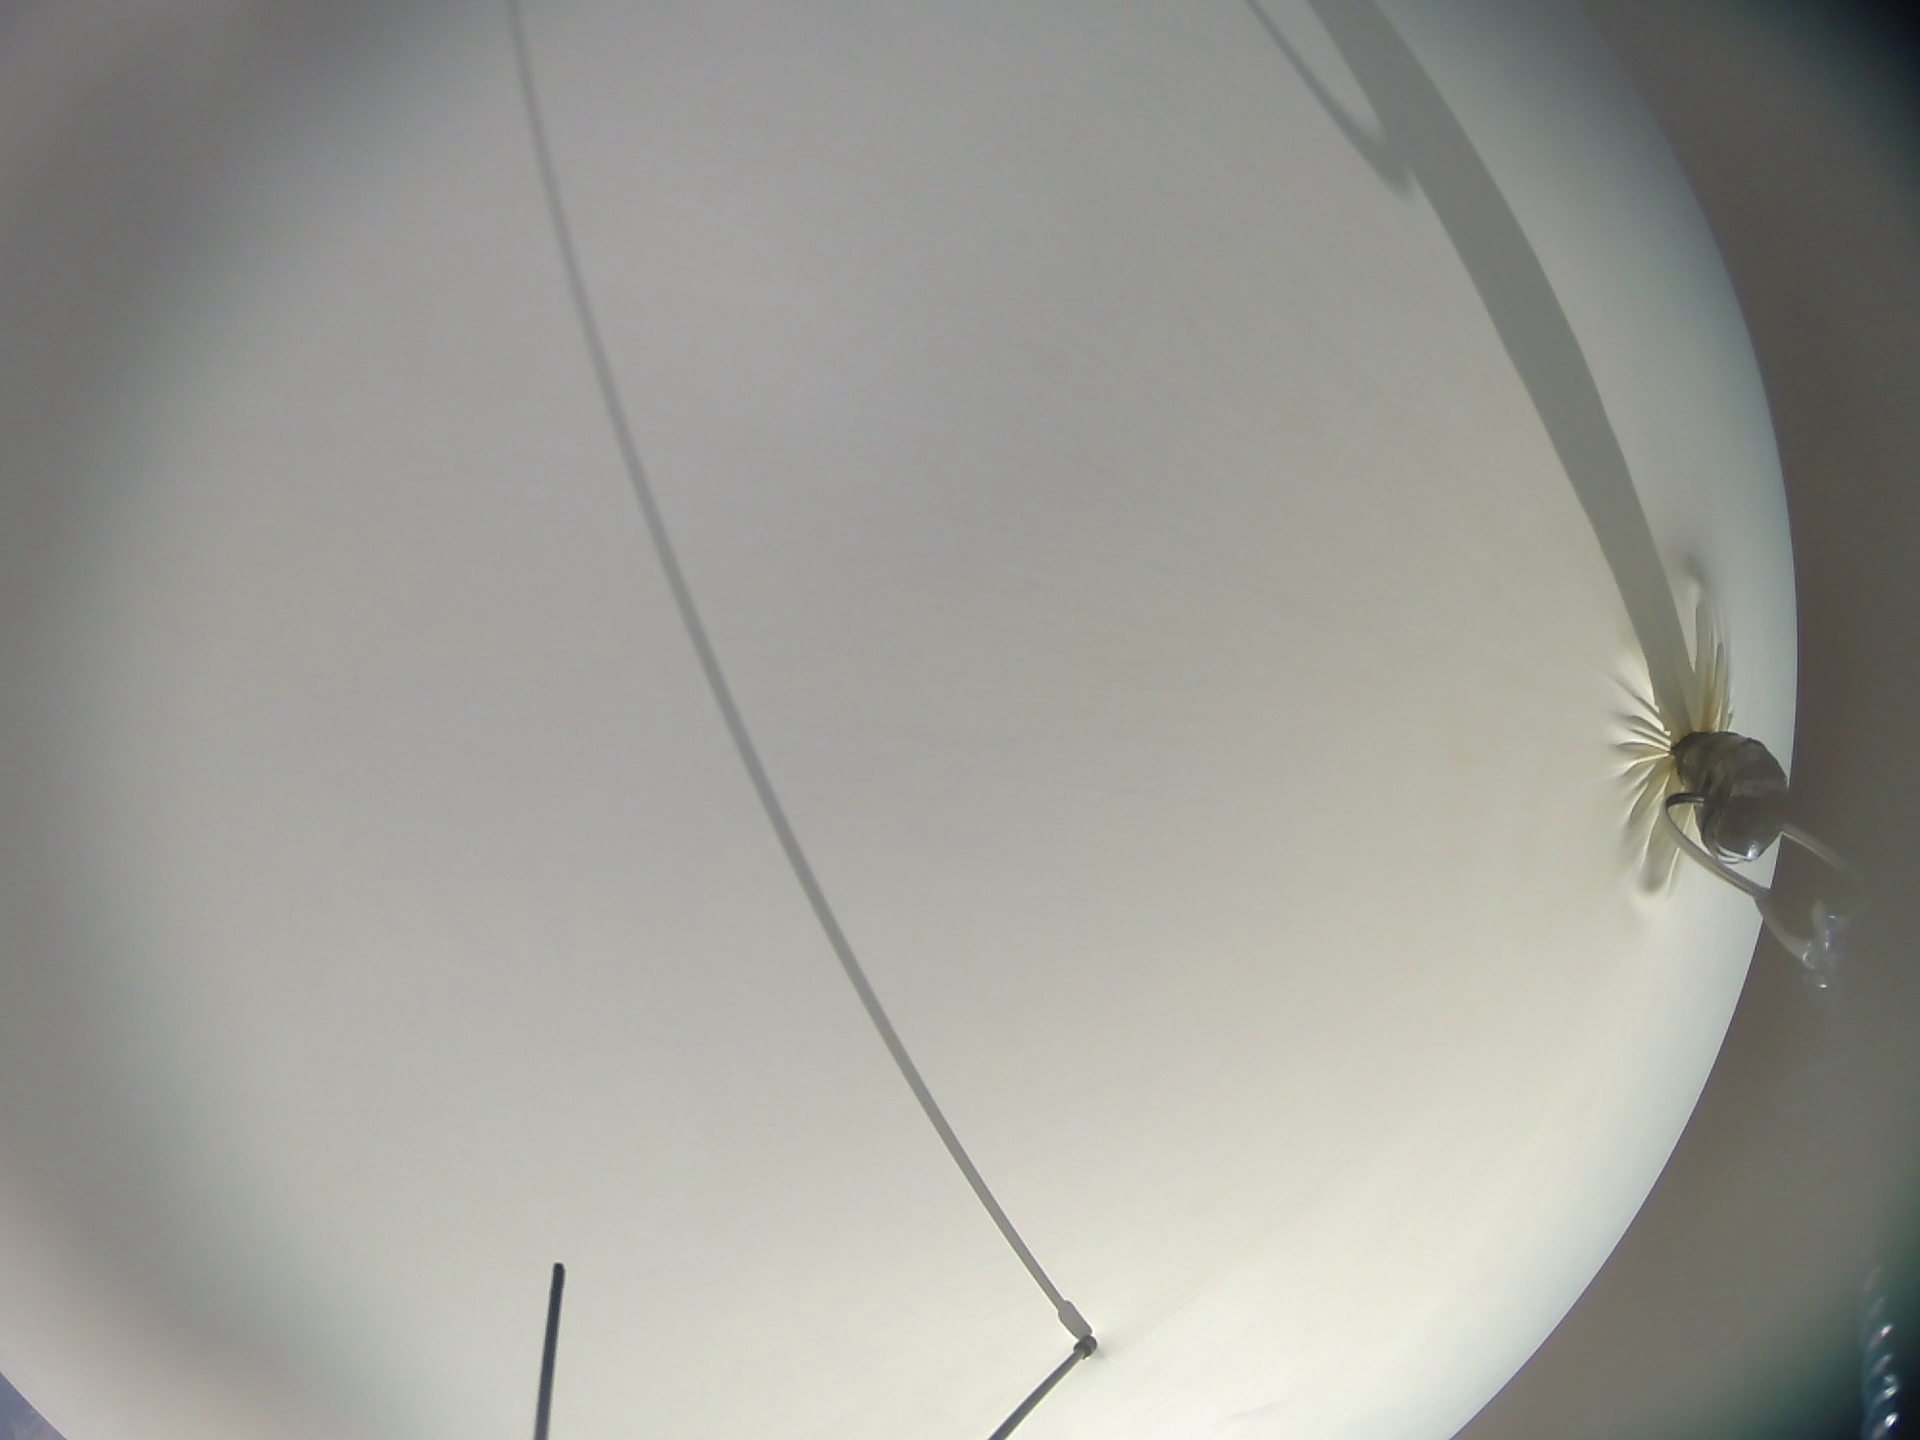
\includegraphics[height=100px]{assets/IMAGEBREAKA} 

}

\caption{\label{fig:figs} APRS antenna touches the surface of teh balloon in the lower middle section of the image.}\label{fig:imagebreaka}
\end{figure}

\begin{figure}[h]

{\centering 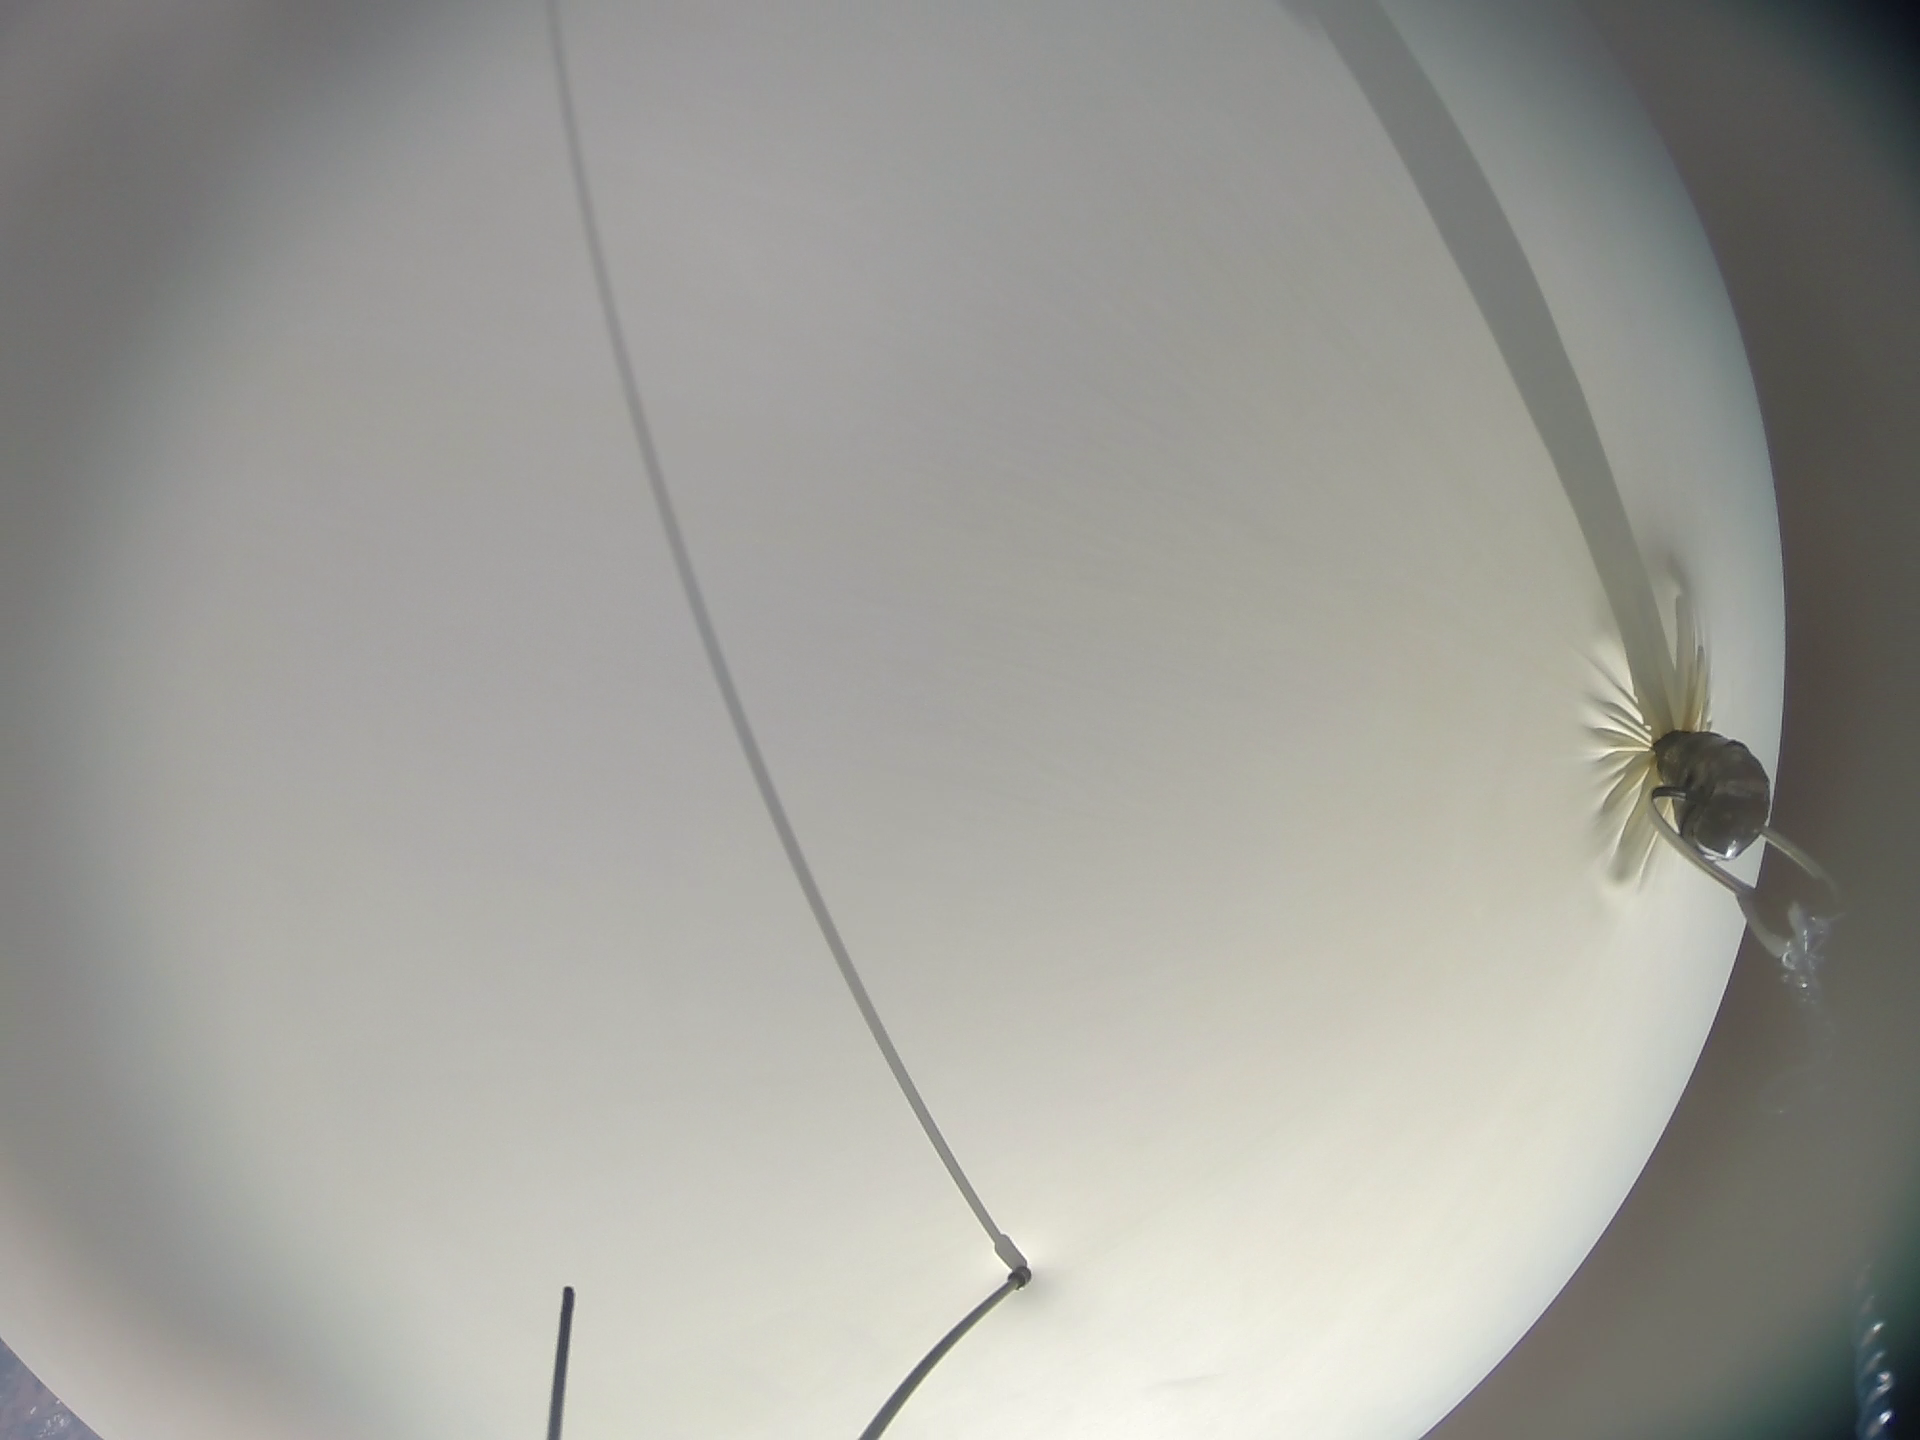
\includegraphics[height=100px]{assets/IMAGEBREAKB} 

}

\caption{\label{fig:figs} APRS antenna applies more pressure on the surface of the balloon.}\label{fig:imagebreakb}
\end{figure}

\begin{figure}[h]

{\centering 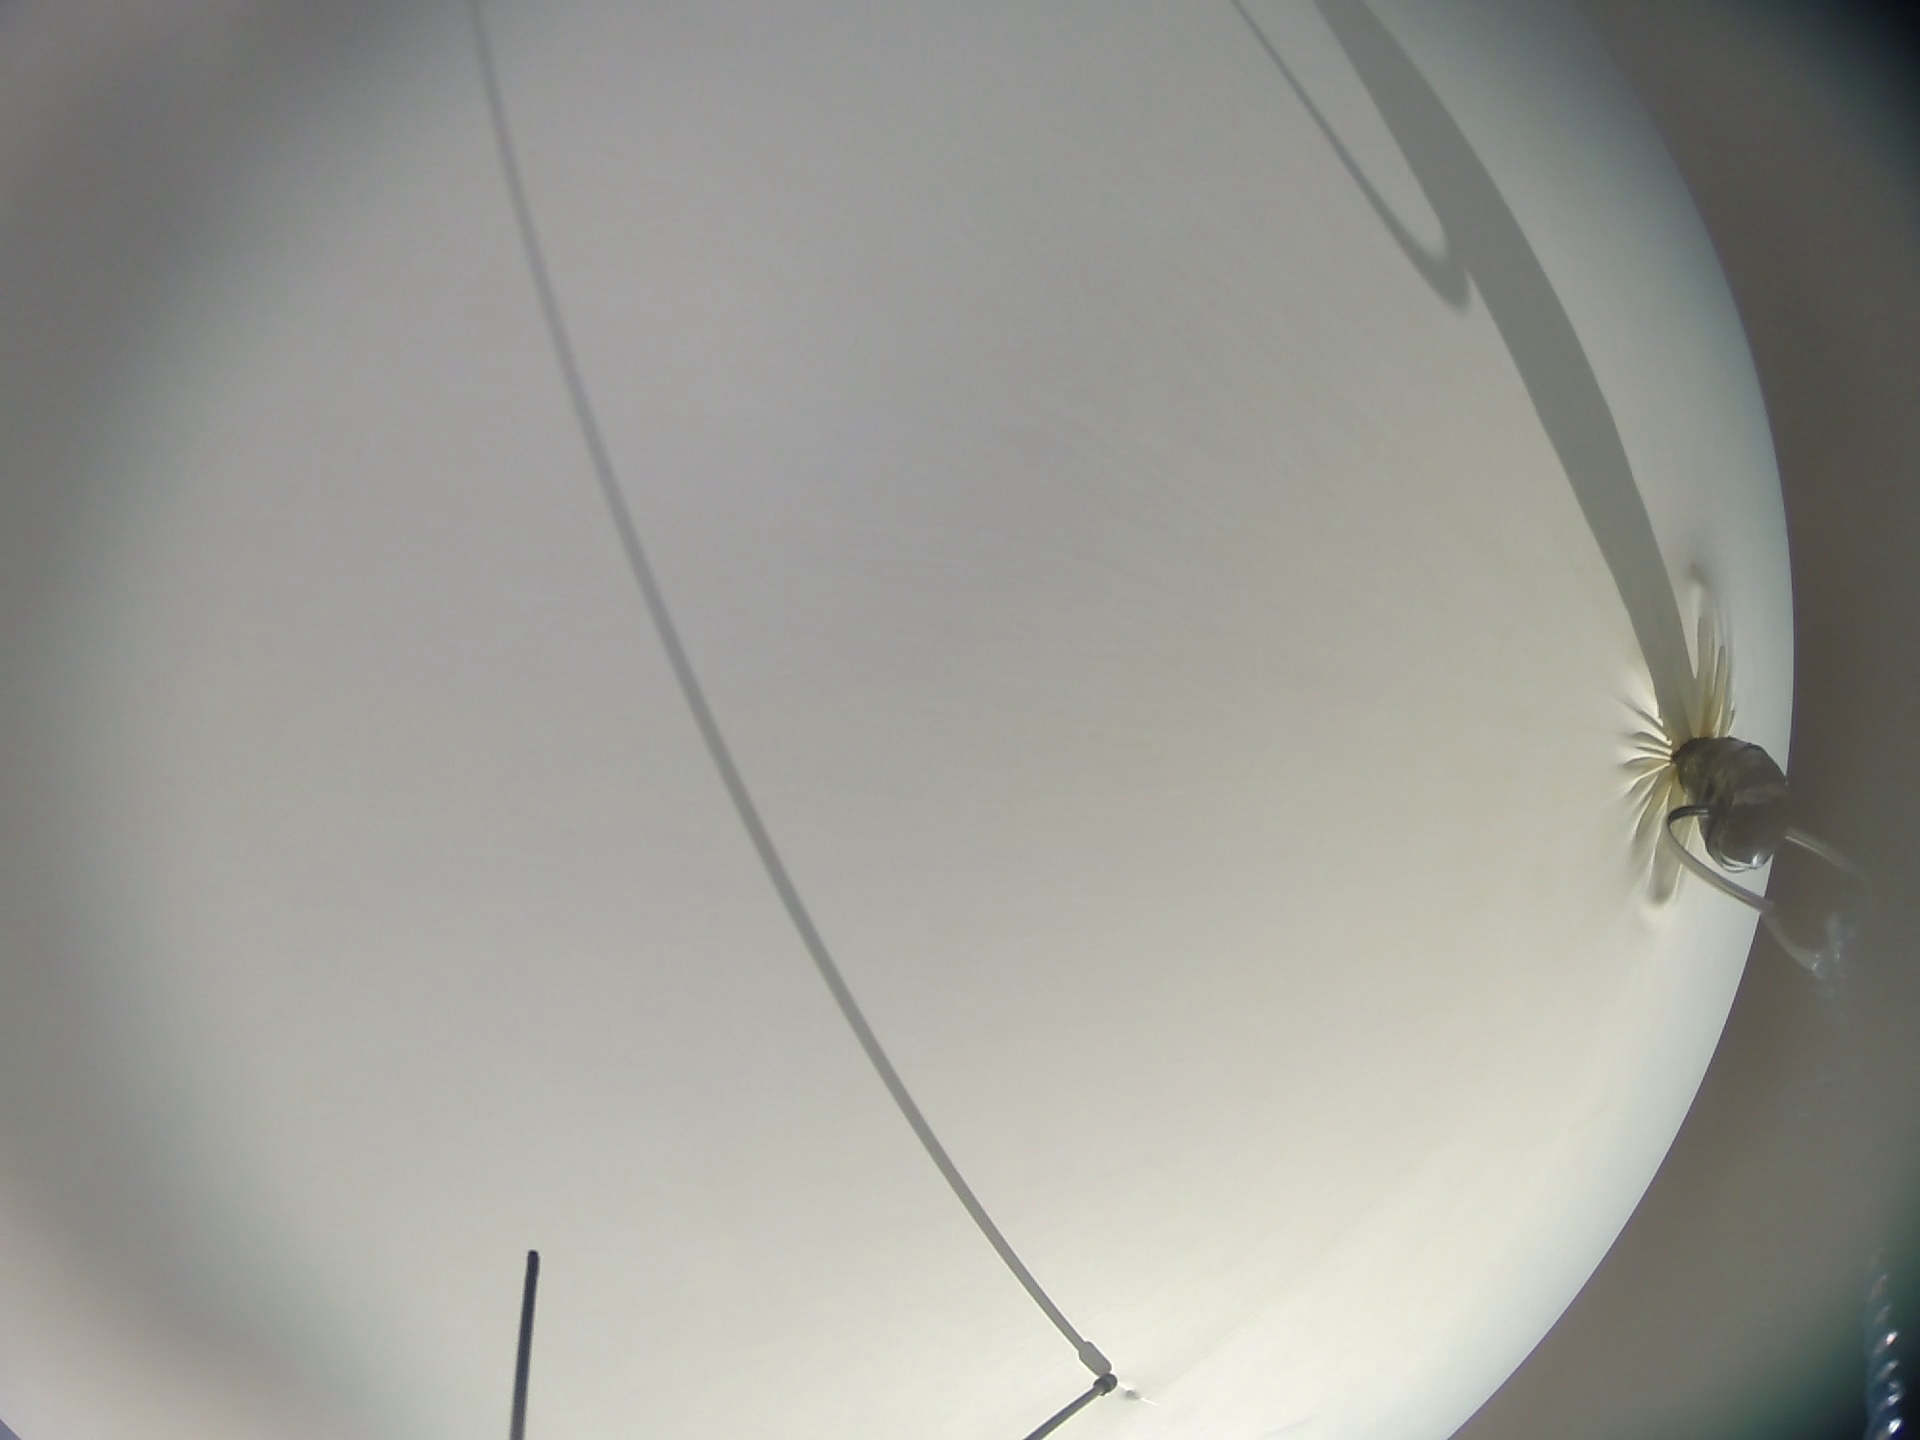
\includegraphics[height=100px]{assets/IMAGEBREAKC} 

}

\caption{\label{fig:figs} Pressure between APRS antenna and balloon is released. A puncture is visible in the balloon.}\label{fig:imagebreakc}
\end{figure}

When the balloon was first popped, the payload began experiencing a
decrease in buoyant force. While the data for when the balloon was at
its peak height is limited, the balloon should likely have accelerated
downwards initially. Around an hour into the flight, the balloon's
decent is not as rapid. This descent rate change is likely due to the
balloon acting like a parachute. The Go-Pro captured a reflection of the
balloon in the payload late into the flight.

\begin{figure}[h]

{\centering 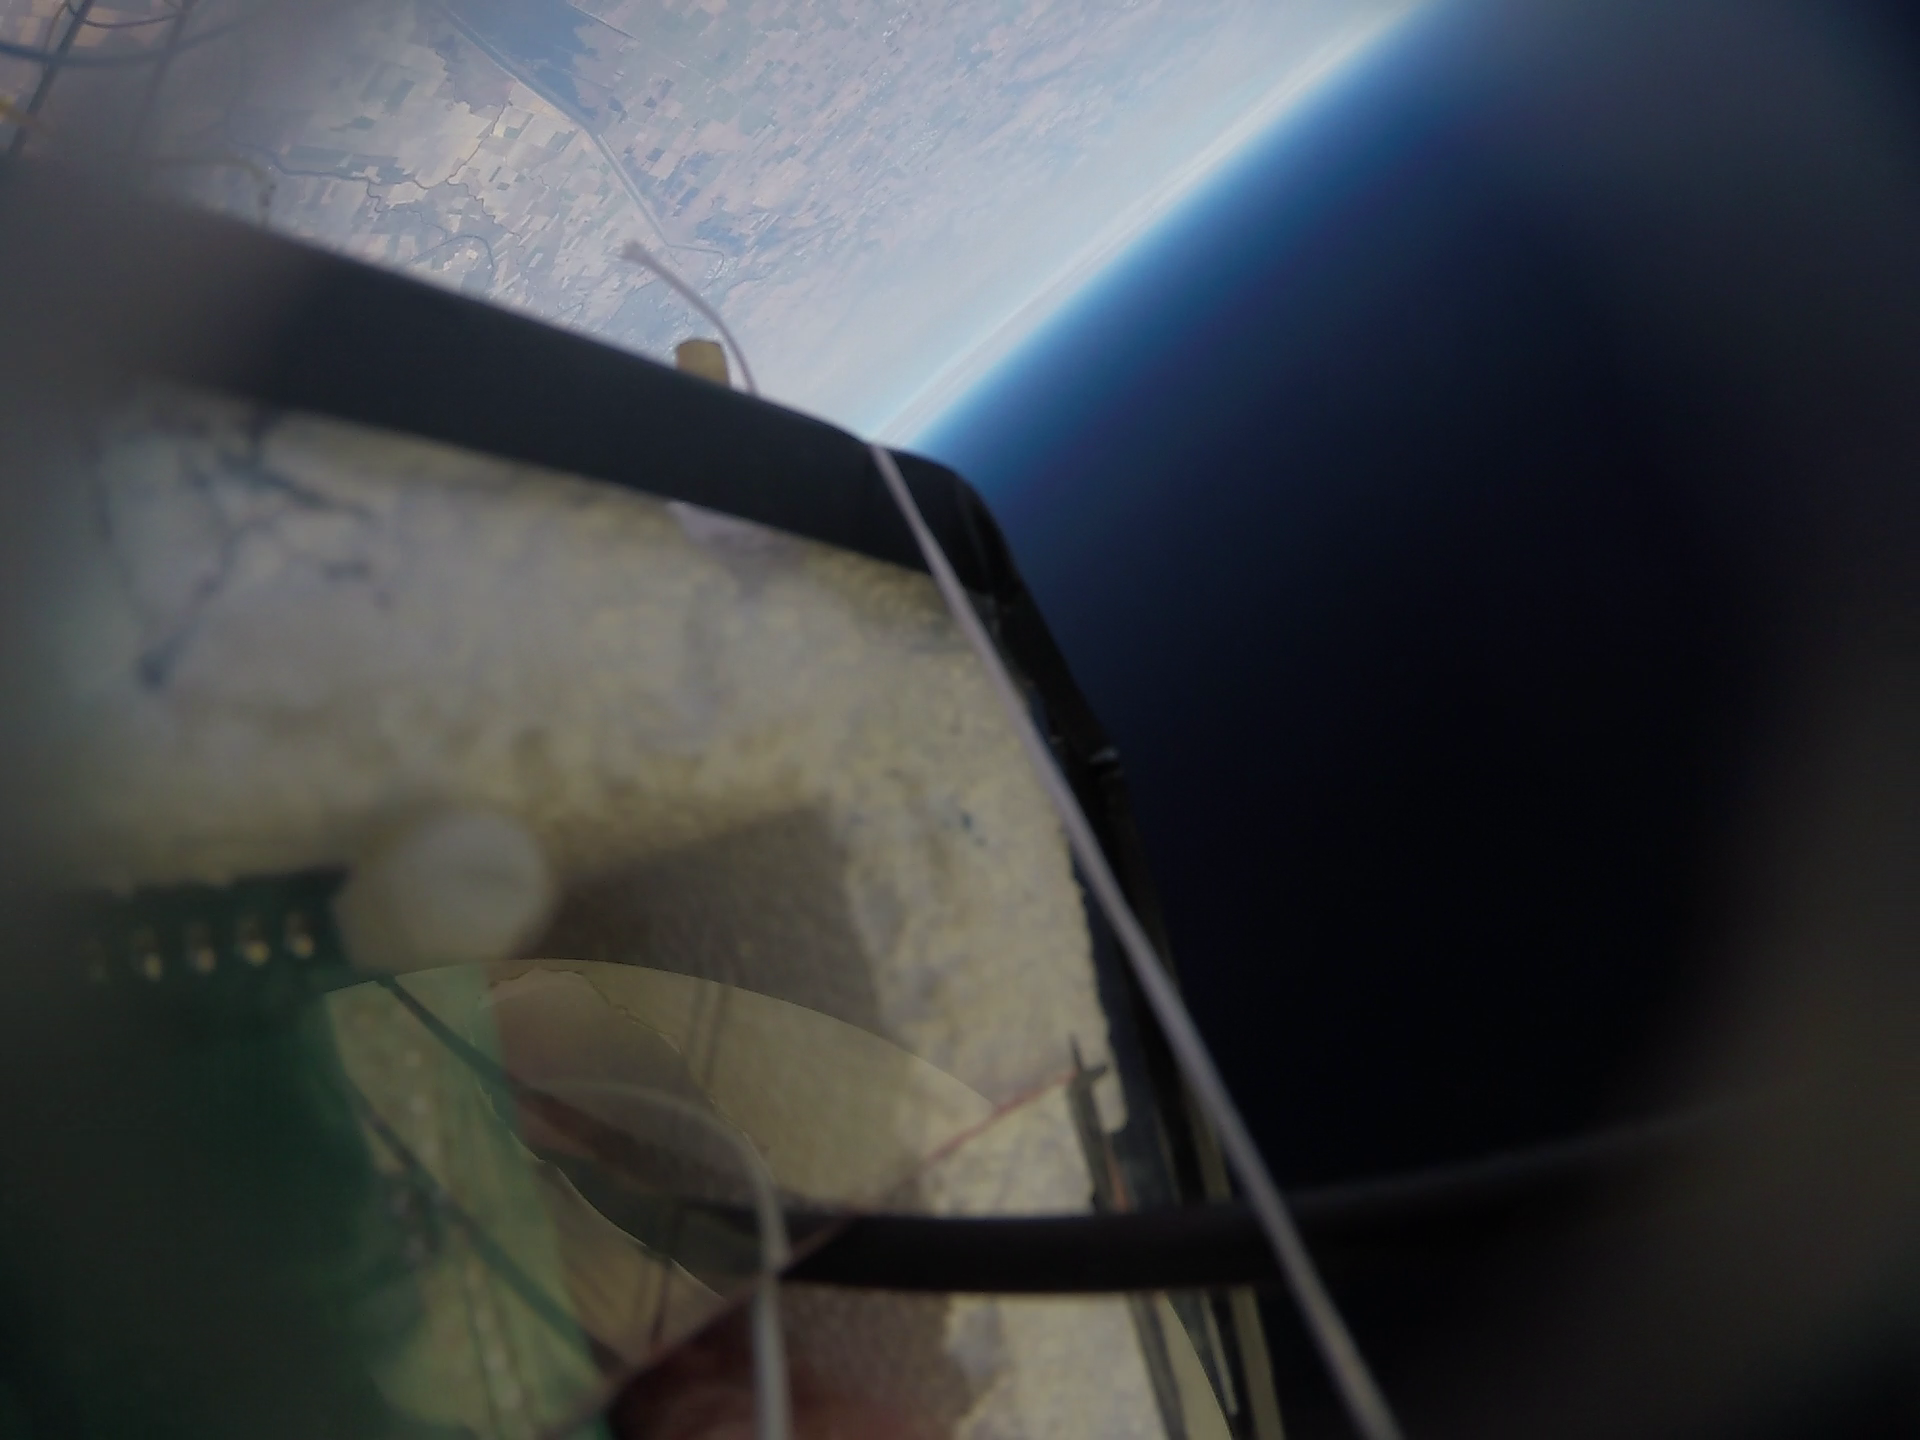
\includegraphics[height=100px]{assets/IMAGEBREAKD} 

}

\caption{\label{fig:figs} Reflection of balloon in payload on lower left side of photo.}\label{fig:imagebreakd}
\end{figure}

The balloons puncture expanded and seems to be capturing air. Since the
balloon acts a parachute, this would increase the air resistance on the
payload and slow down its velocity. At a certain point, the payload
begins descending more rapidly. The parachute affect of the balloon
probably ceased at this point because the ballon was too damaged.

As the balloon entered thicker parts of the atmosphere, the parachute
began becoming more affecting. The rate of falling dramatically slows
down as the payload approaches the surface of the earth.

\subsection{Evaluating NASA's Temperature
Model}\label{evaluating-nasas-temperature-model}

The Arduino BME280 sensor, which was setup to measure outside
temperature, failed quickly, reporting values of -144 \degree C and
100\% Relative Humidity. Therefore, the only metric of temperature
recorded is through the thermistor placed on the sensor PCB in the
payload under the acrylic, which was designed to record the internal
temperature of the payload. This thermistor had little insulation around
it, however, and most likely recorded temperature values closer to the
outside temperature of the atmosphere. The calibrated temperature data
as a function of time is displayed in Figure 11.

\begin{figure}[h]

{\centering 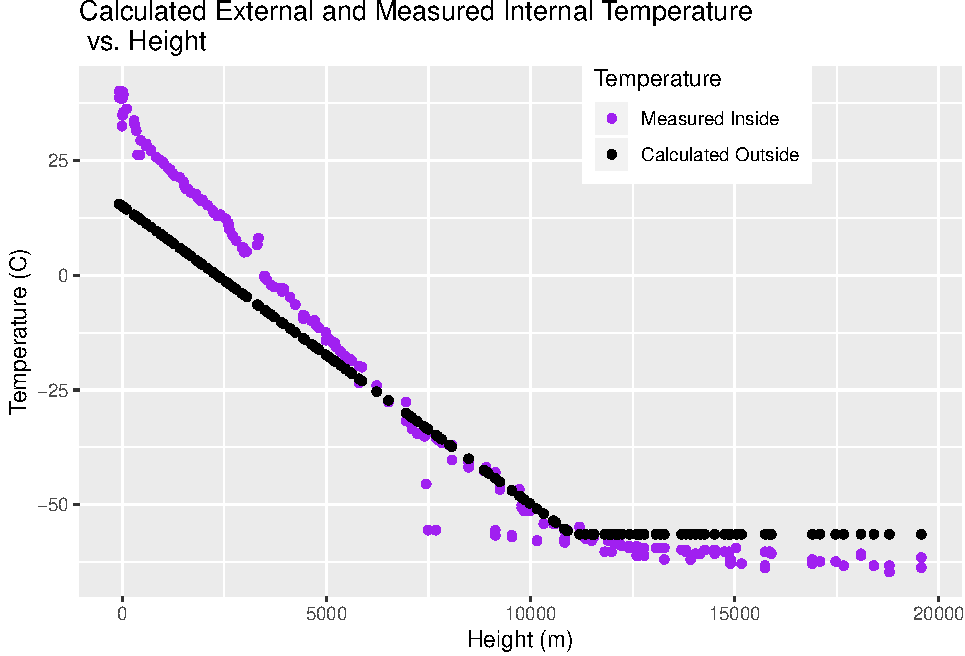
\includegraphics{paper_files/figure-latex/temp_altitude-1} 

}

\caption{\label{fig:figs}}\label{fig:temp_altitude}
\end{figure}

The difference between calculated and actual values can most likely be
explained by the fact that the calibration of the thermistor had a
relatively high error, and there was most likely some insulation keeping
the thermistor warm. Since the balloon never reached the upper
stratosphere at 25,000 meters, no warming effect is observed at high
altitudes. Instead, the temperature stays relatively constant past
11,000 meters in the lower stratosphere before the ozone layer is
reached, since the atmosphere is too thin for much heating infrared
radiation to be absorbed.

The launch was an overall success, other than the BME sensor failing,
Luke Bowsher's accelerometer failing to log data, and the Arduino Mega
failing to log data. Due to the backup tracking system transmitting live
data to the ground, data for all sensors except the accelerometer were
recovered using base station logs.

\section{Conclusion}\label{conclusion}

As discussed, the launch can be considered a technical success. With the
payload and most data recovered, atmospheric analysis has been made
possible by 6thsense's launch. The results discussed above agree with
the scientific community's current understanding of the atmosphere and
atmospheric layers. Not only was data recorded to study the atmosphere,
however, but 6thsense's balloon launch was also a test of systems that
the team designed to meet the technical challenges of sending equipment
to the edge of space.

The 6thsense team, working together for the first time on such a large
project, grew not only their knowledge of the subject matter required to
develop and launch such a payload, but also communication and
collaboration skills, necessary in any large scall venture.


\end{document}
